\documentclass[12pt,a3paper]{article}

%% ── Packages ──────────────────────────────────────────────────────────
\usepackage{amsmath,amssymb}
\usepackage{geometry}
\usepackage{enumitem}
\usepackage{titlesec}
\usepackage[hidelinks,colorlinks=true,linkcolor=blue!70!black]{hyperref}
\usepackage{xcolor}
\usepackage{fancyhdr}
\usepackage{tikz}
\usepackage{chemfig}
\setchemfig{atom sep=4em}
\usepackage{tcolorbox}
\usepackage{multicol}
\usepackage{needspace}
\usepackage[strings]{underscore}
\usepackage{array,booktabs}
\usepackage{tabularx}
\usepackage   [version=4] {mhchem} % for the chemistry
\usepackage{multirow}
\usepackage{fontawesome5}

\usepackage{siunitx}
\usetikzlibrary{intersections, calc}
\usetikzlibrary{arrows.meta, positioning, calc}
\colorlet{mylightblue}{blue!20}
\colorlet{mylightred}{red!10}

\usetikzlibrary{decorations.pathmorphing,calc}
\usetikzlibrary{chains,matrix,positioning}

\usepackage{textcomp}

\tcbuselibrary{skins,breakable}
\geometry{margin=2.5cm,headheight=20pt,top=3cm,bottom=3cm}


\tcbuselibrary{skins,breakable}
% Fix: answer boxes full-width inside enumerate
\tcbset{ansbox/.style={enlarge left by=-\leftmargin, width=\linewidth+\leftmargin}}
\geometry{margin=2.5cm,headheight=20pt,top=3cm,bottom=3cm}


%% ── Colors ────────────────────────────────────────────────────────────
\definecolor{pblue}{RGB}{13,71,161}
\definecolor{dgray}{RGB}{66,66,66}
\definecolor{cA}{RGB}{183,28,28}
\definecolor{cB}{RGB}{1,87,155}
\definecolor{cC}{RGB}{27,94,32}
\definecolor{cD}{RGB}{106,27,154}
\definecolor{cE}{RGB}{230,81,0}
\definecolor{cF}{RGB}{0,96,100}
\definecolor{cG}{RGB}{136,14,79}

%% ── Section headings ──────────────────────────────────────────────────
\titleformat{\section}{\large\bfseries\color{pblue}}{}{0em}{}[\titlerule]

%% ── Header / Footer ───────────────────────────────────────────────────
\pagestyle{fancy}\fancyhf{}
\renewcommand{\headrulewidth}{0.5pt}
\fancyhead[L]{\small\textcolor{pblue}{\textbf{BUET $|$ Chemistry Question Bank}}}
\fancyhead[R]{\small\textcolor{dgray}{\textit{\nouppercase{\leftmark}}}}
\fancyfoot[C]{\small\thepage}

%% ── Utility macros ────────────────────────────────────────────────────
\newcommand{\yr}[1]{\hfill\textcolor{gray}{\small\textbf{[#1]}}}
\newcommand{\mk}[1]{\textcolor{orange!70!black}{\small\textbf{(#1 marks)}}}



\newcommand{\moup}{\textuparrow}
\newcommand{\modown}{\textdownarrow}
\newcommand{\moupdown}{\textuparrow\textdownarrow}

\newcommand{\moupp}{$\uparrow$}
\newcommand{\modownn}{$\downarrow$}
\newcommand{\moupdownn}{$\uparrow\,\downarrow$}


% ── Section divider page ──────────────────────────────────────────────
\newcommand{\secdivider}[4]{%
  \newpage\thispagestyle{empty}%
  \vspace*{\fill}%
  \begin{tcolorbox}[enhanced,colback=#4!7,colframe=#3,boxrule=1.5pt,arc=8pt,
    left=20pt,right=20pt,top=22pt,bottom=22pt,
    shadow={3pt}{-3pt}{0pt}{black!15}]
    \centering
    {\large\textcolor{gray}{\textbf{BUET $\cdot$ CHEM 113}}}\\[8pt]
    {\fontsize{26}{32}\selectfont\bfseries\textcolor{#3}{Chemistry}}\\[6pt]
    {\fontsize{15}{19}\selectfont\textcolor{dgray}{#1}}\\[12pt]
    \textcolor{#3!60}{\rule{0.5\textwidth}{0.5pt}}\\[6pt]
    {\small\textcolor{gray}{#2}}
  \end{tcolorbox}%
  \vspace*{\fill}\newpage%
}




%% ── List styles ───────────────────────────────────────────────────────
\setlist[enumerate,1]{label=\textbf{Q\arabic*.},leftmargin=*,itemsep=14pt,parsep=2pt}
\setlist[enumerate,2]{label=(\alph*),leftmargin=2em,itemsep=3pt}
\setlist[enumerate,3]{label=(\roman*),leftmargin=2.5em,itemsep=2pt}

%% ══════════════════════════════════════════════════════════════════════
\begin{document}

%% ── COVER ─────────────────────────────────────────────────────────────
\thispagestyle{empty}
\begin{tcolorbox}[enhanced,colback=cB!5,colframe=cB,boxrule=1.5pt,arc=6pt,
  top=28pt,bottom=28pt,left=22pt,right=22pt,
  shadow={4pt}{-4pt}{0pt}{black!20}]
  \centering

    
\includegraphics[height=2.5cm]{images/buet_logo.png}\\[8pt]

  {\Large\bfseries\textcolor{cB}{Bangladesh University of Engineering and Technology}}\\[4pt]
  {\normalsize\textcolor{dgray}{Department of Computer Science \& Engineering}}\\[18pt]
  \textcolor{cB}{\rule{\textwidth}{1pt}}\\[14pt]
  {\fontsize{22}{28}\selectfont\bfseries\textcolor{cB}{CHEM 113 Question Bank}}\\[8pt]
  {\fontsize{14}{18}\selectfont\textcolor{dgray}{Chemistry}}\\[4pt]
  {\normalsize\textcolor{dgray}{CHEM 113 / CHEM 101 \quad (L-1/T-2)}}\\[18pt]
  \textcolor{cB}{\rule{\textwidth}{0.5pt}}\\[14pt]
  {\small\textcolor{dgray}{Year Coverage:\;2006--07 to 2023--24 \\ Topics:\;Quantum Mechanics, Bonding, Solutions, Colloids, Phase Diagrams, Electrochemistry \& more}}\\[16pt]
  \begin{center}
    {\small\bfseries\textcolor{dgray}{Authors \& Contributors}}\\[6pt]
    \begin{tabular}{rl}
      \textbf{Md Ratul Hasan} \textcolor{dgray}{\small(2405009)} & --- Question Curation \& Organisation\\
      & --- \LaTeX\ Typesetting\\[3pt]
      \textbf{NotebookLM} & --- Research \& Extraction\\[3pt]
      \textbf{Claude AI}  & --- \LaTeX\ Typesetting\\[3pt]
      \textbf{ChatGPT}    & --- Prompt\\
    \end{tabular}
  \end{center}
\end{tcolorbox}
\newpage

%% ── TABLE OF CONTENTS ─────────────────────────────────────────────────
\thispagestyle{fancy}\markboth{Table of Contents}{}
\begin{center}
  {\LARGE\bfseries\textcolor{pblue}{Table of Contents}}\\[6pt]
  \textcolor{pblue}{\rule{0.6\textwidth}{0.8pt}}
\end{center}
\vspace{6pt}

\begin{tcolorbox}[colback=cA!5,colframe=cA,boxrule=1pt,arc=5pt,
  left=8pt,right=8pt,top=8pt,bottom=8pt,before skip=4pt]
  {\large\bfseries\textcolor{cA}{Part I --- Atomic \& Molecular Theory}}\\[5pt]
  \textcolor{cA!40}{\rule{\textwidth}{0.4pt}}\\[3pt]
  \small\begin{itemize}[leftmargin=1.2em,itemsep=1pt,label={\textcolor{cA}{$\triangleright$}}]
    \item \hyperref[sec:S1]{\textbf{S1.} Quantum Concept \& Atomic Structure}
    \item \hyperref[sec:S2]{\textbf{S2.} Molecular Geometry}
    \item \hyperref[sec:S3]{\textbf{S3.} Chemical Bonding}
  \end{itemize}
\end{tcolorbox}

\begin{tcolorbox}[colback=cB!5,colframe=cB,boxrule=1pt,arc=5pt,
  left=8pt,right=8pt,top=8pt,bottom=8pt,before skip=4pt]
  {\large\bfseries\textcolor{cB}{Part II --- Solution Chemistry}}\\[5pt]
  \textcolor{cB!40}{\rule{\textwidth}{0.4pt}}\\[3pt]
  \small\begin{itemize}[leftmargin=1.2em,itemsep=1pt,label={\textcolor{cB}{$\triangleright$}}]
    \item \hyperref[sec:S4]{\textbf{S4.} Properties of Solutions}
    \item \hyperref[sec:S5]{\textbf{S5.} Colloid \& Nanochemistry}
    \item \hyperref[sec:S6]{\textbf{S6.} Phase Rule \& Phase Diagram}
  \end{itemize}
\end{tcolorbox}

\begin{tcolorbox}[colback=cC!5,colframe=cC,boxrule=1pt,arc=5pt,
  left=8pt,right=8pt,top=8pt,bottom=8pt,before skip=4pt]
  {\large\bfseries\textcolor{cC}{Part III --- Energy \& Electrochemistry}}\\[5pt]
  \textcolor{cC!40}{\rule{\textwidth}{0.4pt}}\\[3pt]
  \small\begin{itemize}[leftmargin=1.2em,itemsep=1pt,label={\textcolor{cC}{$\triangleright$}}]
    \item \hyperref[sec:S7]{\textbf{S7.} Energy \& Chemistry}
    \item \hyperref[sec:S8]{\textbf{S8.} Electrochemistry}
  \end{itemize}
\end{tcolorbox}

\begin{tcolorbox}[colback=cD!5,colframe=cD,boxrule=1pt,arc=5pt,
  left=8pt,right=8pt,top=8pt,bottom=8pt,before skip=4pt]
  {\large\bfseries\textcolor{cD}{Part IV --- Advanced Topics}}\\[5pt]
  \textcolor{cD!40}{\rule{\textwidth}{0.4pt}}\\[3pt]
  \small\begin{itemize}[leftmargin=1.2em,itemsep=1pt,label={\textcolor{cD}{$\triangleright$}}]
    \item \hyperref[sec:S9]{\textbf{S9.} Polymers}
    \item \hyperref[sec:S10]{\textbf{S10.} Electronic Materials}
    \item \hyperref[sec:S11]{\textbf{S11.} Biomolecules}
    \item \hyperref[sec:S12]{\textbf{S12.} Computational Chemistry}
    \item \hyperref[sec:S13]{\textbf{S13.} Miscellaneous}
  \end{itemize}
\end{tcolorbox}

\newpage

%%══════════════════════════════════════════════════════════════════════
%% S1 — Quantum Concept & Atomic Structure
%%══════════════════════════════════════════════════════════════════════
\secdivider{Section S1}{Quantum Concept \& Atomic Structure}{cA}{cA}
\markboth{S1 --- Quantum Concept \& Atomic Structure}{}

  \label{sec:S1}
\section{S1 --- Quantum Concept \& Atomic Structure}

\begin{enumerate}
\item Explain why each element having a characteristic emission and absorption spectra is significant in understanding dual nature of electron? \mk{5--10}
\yr{CHEM 113 | 2023--24; 2020--21}



\item Describe the relationship between electron shielding and $Z_{\text{eff}}$ on the outermost electrons of an atom. Predict how chemical reactivity is affected by a decreased effective nuclear charge. \mk{5--10}
\yr{CHEM 113 | 2020--21; 2022--23; 2023--24}



\item Analyze the radial distribution functions for the hydrogenic 1s, 2s, and 2p orbitals, clearly illustrating their nodal structures. Based on your analysis, justify why the electron in the 2s orbital exhibits a greater probability of being found closer to the nucleus compared to the 2p orbital. \mk{10}
\yr{CHEM 113 | 2023--24}





\item Evaluate the case of a Ca$^{19+}$ ion with its electron in the 6th excited state: (i) Calculate the longest wavelength of light emitted when the electron transitions to a lower energy level. (ii) Suppose the same transition as in part (i) took place in a hydrogen atom. Would the wavelength of emission be longer than, shorter than, or the same as your answer? \mk{10}
\yr{CHEM 113 | 2023--24}



\item Discuss the periodic trends in ionization energy, electron affinity, atomic size, and metallic properties of elements, illustrating your explanation with the help of a labeled outline of the periodic table. \mk{10}
\yr{CHEM 113 | 2023--24}




\item Consider a photoelectric experiment in which light of variable frequency strikes a metal surface. Plot the kinetic energy of emitted electrons as a function of the frequency of the incident light. From this graph, derive the work function of the metal, and discuss how the graph would differ if the light source were replaced with a source of lower frequency which is below the threshold frequency. \mk{10}
\yr{CHEM 113 | 2022--23}



\item Inside an atom, the uncertainty in the position of an electron is 0.1 nm. Calculate the minimum uncertainty in the momentum of the particle. If the electron has a de Broglie wavelength $\lambda = 2.0 \times 10^{-10}$ m, calculate its velocity and discuss how the uncertainty in the particle's position influences its momentum and velocity. \mk{10}
\yr{CHEM 113 | 2022--23}



\item Sketch the wave functions and the probabilities for 3s, 3p, and 4s orbitals. \mk{5}
\yr{CHEM 113 | 2022--23}



\item Demonstrate the relationship between blackbody radiation and Planck's quantum theory. \mk{10}
\yr{CHEM 113 | 2021--22}



\item Concisely describe the physical significance of $\Psi^2$ for a hydrogen atom. \mk{5}
\yr{CHEM 113 | 2021--22}



\item Plot the radial probability distribution for a 2s orbital (as a solid line) and a 2p orbital (as a dashed line). For each orbital indicate any radial nodes with an arrow. Compare the shielding experienced by a 2s electron to that of a 2p electron and provide a brief explanation. \mk{10}
\yr{CHEM 113 | 2021--22}



\item Consider a Ca$^{19+}$ ion with its electron in the 5th excited state. (i) Calculate the longest wavelength of light that could be emitted when the Ca$^{19+}$ electron transitions to a lower energy state. (ii) Suppose the same transition as in part (i) took place in a hydrogen atom. Would the wavelength of emission be longer than, shorter than, or the same as your answer? \mk{10}
\yr{CHEM 113 | 2021--22}



\item Explain why elements produce their own characteristic colors when they emit photons. How is the concept of electron density used to describe the motions and energies of submicroscopic particles in the quantum mechanical treatment of an atom? \mk{15}
\yr{CHEM 113 | 2020--21 (Jan 21)}



\item What role did Einstein's explanation of the photoelectric effect play in the development of the particle-wave interpretation of the nature of electromagnetic radiation? Does a baseball in motion possess wave properties? If so, why can we not determine its wave properties? \mk{20}
\yr{CHEM 113 | 2020--21 (Jan 21)}



\item Show the radial distribution function for hydrogenic 1s, 2s and 2p orbitals with nodes. Why does 2s give the electron a greater probability of close approach to the nucleus compared to 2p orbital? \mk{10}
\yr{CHEM 113 | 2020--21}



\item In making a transition from an orbital with a principal quantum number of 4 to an orbital with a principal quantum number of 7, does the electron of a hydrogen atom emit or absorb a photon of energy? What would be the energy of the photon? To what region of the electromagnetic spectrum does this energy correspond? \mk{10}
\yr{CHEM 113 | 2020--21}



\item Account for the large decrease in electron affinity between Li and Be despite the increase in nuclear charge? \mk{5}
\yr{CHEM 113 | 2020--21}



\item How is the concept of electron density used to describe the position of an electron in the quantum mechanical treatment of an atom? \mk{7--15}
\yr{CHEM 113 | 2017--18; 2019--20}



\item Point out three characteristic features in the photoelectric effect that cannot be explained on the basis of wave theory of light. Provide a brief explanation of those features. \mk{15}
\yr{CHEM 113 | 2019--20}



\item The wave nature of matter is not noticeable in our daily observations --- Why? \mk{5}
\yr{CHEM 113 | 2017--18}



\item Describe the experimental basis for believing that the electrons in an atom behave as tiny bar magnets. \mk{15}
\yr{CHEM 113 | 2017--18}



\item Describe the role played in elucidating the atomic structures by each of the following: (i) Positive rays, (ii) Cathode rays, (iii) X-rays. \mk{18}
\yr{CHEM 113 | 2017--18}



\item Crystal diffraction can be studied by electron diffraction as well as by neutron diffraction method. What should be the ratio of the velocities of electron and neutron for the de Broglie wavelength to be the same? (You don't need to use any data to solve this problem.) \mk{5}
\yr{CHEM 113 | 2017--18}



\item Schr\"{o}dinger equation can be represented in a simpler form as $H\Psi = E\Psi$, where $E$ is the energy and $\Psi$ is called a wave function. What information can you get from the equation about an electron in an atom? \mk{6}
\yr{CHEM 113 | 2016--17}



\item Justify the statement: ``The probability of finding two electrons with the same four quantum numbers in an atom is zero.'' \mk{10}
\yr{CHEM 113 | 2016--17}



\item The He$^+$ ion contains only one electron and is therefore hydrogen-like. Calculate the wavelength, in increasing order, of the first four transitions in the Balmer series of the He$^+$ ion. Compare these wavelengths with the same transitions in an H atom. Comment on the differences. (The Rydberg constant for He$^+$ is $8.72 \times 10^{-18}$ J and that for H is $2.18 \times 10^{-18}$ J.) \mk{9}
\yr{CHEM 113 | 2016--17}



\item What are photons? What role did Einstein's explanation of the photoelectric effect play in the development of the particle-wave interpretation of the nature of electromagnetic radiation? \mk{9--12}
\yr{CHEM 113 | 2015--16; 2011--12}



\item What do you mean by Eigen values and Eigen functions? \mk{6--8}
\yr{CHEM 113 | 2015--16; 2011--12}



\item The electron in the hydrogen atom makes a transition from an energy state of principal quantum number $n_i$ to the $n=2$ state. If the photon emitted has a wavelength of 434 nm, what is the value of $n_i$? \mk{7--8}
\yr{CHEM 113 | 2015--16; 2014--15}



\item Matter and radiation have a ``dual nature'' --- Explain. \mk{5}
\yr{CHEM 113 | 2015--16}



\item What is meant by the term ``Shielding of electrons'' in an atom? Using the Li atom as an example, describe the effect of shielding on the energy of electrons in an atom. \mk{7}
\yr{CHEM 113 | 2015--16}



\item In your own words, explain the photoelectric effect.\mk{4}\yr{CHEM 113 | 2014--15}



\item The binding energy of an electron in a metal surface is $5.86 \times 10^{-19}$ J. (i) Calculate the minimum frequency of light required to release electrons from the metal. (ii) Calculate the kinetic energy of the ejected electron if light frequency $2.00 \times 10^{15}$ s$^{-1}$ is used for irradiating the metal ($h = 6.63 \times 10^{-34}$ J$\cdot$s). \mk{6}
\yr{CHEM 113 | 2014--15}



\item What is meant by the term ``Effective nuclear charge ($Z_{\text{eff}}$)'' in an atom? Using the Sodium ($z = 11$) atom as an example, describe the effect of shielding on the 1st ionization energy. \mk{4}
\yr{CHEM 113 | 2014--15}



\item Describe how you build up the detailed electron configuration with the help of all four quantum numbers. \mk{10}
\yr{CHEM 113 | 2014--15}



\item Draw a rough sketch of a periodic table (no details required). Indicate where alkali metals, chalcogens and halogens are located. Write the name and symbol for an element in each of these groups. \mk{--}
\yr{CHEM 113 | 2014--15}



\item Explain with a figure how each of these properties of the representative elements generally increases or decreases across the periodic table: (i) atomic size, (ii) electron affinity, (iii) ionization energy, (iv) metallic character, (v) acidity of oxides. \mk{12}
\yr{CHEM 113 | 2014--15}



\item Give a brief description of the wave nature of light. What are the two main characteristics of light wave?\mk{4}
\yr{CHEM 113 | 2014-15}



\item Give the equiation that relates wave-particle properties of light. Explain the meaning of each symbol in the equation.\mk{4}
\yr{CHEM 113 | 2014-15}



\item What is Heisenberg's Uncertainty principle? Prove that the product of uncertainty in position of an electron with uncertainty in momentum of the same electron is of the order of Planck's constant. \mk{11}
\yr{CHEM 113 | 2013--14}



\item Draw emission spectra of hydrogen atom. Why does a hydrogen atom give so many lines in its spectrum although there is only one electron in it? \mk{8}
\yr{CHEM 113 | 2012--13}



\item Derive the equation by which you can calculate the wavelength of a line in the hydrogen spectrum. Calculate the wavelength of the line in the Brackett series of hydrogen spectrum that is associated with a drop of the electron from the 7th orbit. (Rydberg constant $= 1097\,\text{m}^{-1}$) \mk{17}
\yr{CHEM 113 | 2012--13}



\item Give a brief account of the wave--particle duality nature of the electron. \mk{10}
\yr{CHEM 113 | 2012--13}




\item Group the species that are isoelectronic: Be$^{2+}$, F$^-$, Fe$^{2+}$, N$^{3-}$, He, S$^{2-}$, Co$^{3+}$, Ar. \mk{8}
\yr{CHEM 113 | 2011--12}



\item Ionization energy is usually measured in the gaseous state. Why? \mk{7}
\yr{CHEM 113 | 2011--12}



\item What are the limitations of Bohr's atomic theory? \mk{4}
\yr{CHEM 113 | 2011--12}



\item State the general periodic trends in size of atomic radii. Arrange the following atoms in order of decreasing atomic radius: Na, Al, P, Cl, Mg. \mk{9}
\yr{CHEM 113 | 2011--12}



\item Derive an expression applying Bohr atom model for the calculation of wavelength of radiation obtained in the emission spectrum of hydrogen. \mk{10}
\yr{CHEM 101 | 2010--11}



\item What does Schr\"{o}dinger wave equation describe? Deduce the equation and comment on its solution. \mk{10}
\yr{CHEM 101 | 2010--11}



\item Mention the variations of the following properties of the elements within periods and groups in the periodic table and give reasons for these variations: (i) Oxidation power, (ii) Metallic character, (iii) Ionic radii, (iv) Reducing power, (v) Atomic size. \mk{7}
\yr{CHEM 101 | 2010--11}



\item Calculate the magnitude of energy in erg of a quantum associated with light of wavelength 60.0 \AA. \mk{8}
\yr{CHEM 101 | 2010--11}



\item What is quantum theory of radiation? Discuss photoelectric effect in relation to quantization of energy. \mk{10}
\yr{CHEM 101 | 2009--10}



\item What are the limitations of Bohr's atomic theory and how are they overcome? \mk{10}
\yr{CHEM 101 | 2009--10}



\item Justify the stability of a nucleus of an atom. \mk{8}
\yr{CHEM 101 | 2009--10}



\item What is periodic law? How many periods and groups are there in a periodic table? Why are the periods not equal? \mk{8}
\yr{CHEM 101 | 2009--10}



\item How would you conceive the idea of having an electron cloud around the nucleus of an atom? How is it experimentally proved that the electron has wave nature? \mk{11}
\yr{CHEM 101 | 2009--10}



\item Deduce an equation by which the propagation of electron wave in space can be described. How can the solutions of the equation be used to describe the different shapes of orbitals? \mk{12}
\yr{CHEM 101 | 2009--10}



\item What are the transition elements and which periods of the periodic table do they belong to? Discuss the important properties of transition elements. \mk{7}
\yr{CHEM 101 | 2008--09}



\item What are noble gases? Discuss the important physical and chemical properties of noble gases. \mk{7}
\yr{CHEM 101 | 2008--09}



\item Discuss the quantum theory of radiation. How is Planck's hypothesis for radiation of energy related to the spectral properties of an atom described by Bohr? \mk{13}
\yr{CHEM 101 | 2008--09}



\item What are the limitations of Bohr's atomic structure? How was the structure modified by Sommerfeld? \mk{10}
\yr{CHEM 101 | 2008--09}



\item Deduce de Broglie's equation. Explain with suitable examples the physical significance of the equation. \mk{11}
\yr{CHEM 101 | 2008--09}



\item State Heisenberg's Uncertainty principle. Show that the uncertainty principle is applicable only for small particles like the electron. \mk{9}
\yr{CHEM 101 | 2007--08}



\item Discuss the classification of the elements present in the periodic table on the basis of electronic configuration. Mention the characteristics of two important classes of elements. \mk{15}
\yr{CHEM 101 | 2007--08}




%%══════════════════════════════════════════════════════════════════════
%% S2 — Molecular Geometry
%%══════════════════════════════════════════════════════════════════════
\item What are the postulates of Bohr's atomic model? Based on the postulates, deduce an equation for the calculation of the difference in energies between two levels for an electron in an atom. How far is the Bohr model successful in explaining the spectral properties of an atom? \mk{17}
\yr{CHEM 101 | 2006--07}



\item What is the general electronic configuration of transition elements? Discuss the general properties of transition elements. \mk{10}
\yr{CHEM 101 | 2006--07}



\item Deduce de Broglie's equation. With a suitable example, discuss the applicability of the equation in the case of electron-like particles. \mk{9}
\yr{CHEM 101 | 2006--07}



\item How would you conceive the idea of having an electron cloud around the nucleus of an atom? \mk{6}
\yr{CHEM 101 | 2006--07}


\end{enumerate}
\newpage

\secdivider{Section S2}{Molecular Geometry}{cB}{cB}
\markboth{S2 --- Molecular Geometry}{}
  \label{sec:S2}
\section{S2 --- Molecular Geometry}

\begin{enumerate}
\item Predict the shapes of (i) SO$_3^{2-}$ and (ii) PCl$_4^+$ ions showing all the necessary steps. \mk{10}
\yr{CHEM 113 | 2020--21}



\item Sketch the shape or three-dimensional structure of each of the following: BrO$_3^-$ and AsF$_4^-$. Name the shapes and state the status of hybridization in the central atoms. \mk{6}
\yr{CHEM 113 | 2017--18}



\item Draw the trigonal bipyramidal geometry and mark the axial and equatorial positions. Which position is suitable for the accommodation of a lone pair in the system? Why? \mk{6}
\yr{CHEM 113 | 2016--17}



\item Draw the geometry of the following and predict the angles: (i) PO$_4^{3-}$ (ii) I$_3^-$. \mk{6}
\yr{CHEM 113 | 2016--17}



\item How does VBT apply the concept of hybridization? Illustrate the hybridization process of water. \mk{9}
\yr{CHEM 113 | 2016--17}



\item Use the VSEPR model to predict the geometry of the following ions: (i) N$_3^-$ (ii) BH$_4^-$ (iii) SO$_3^{2-}$ (iv) NO$_2^-$. \mk{8}
\yr{CHEM 113 | 2015--16}



\item In the trigonal bipyramidal arrangement for a system AB$_4$E, why does the lone pair occupy an equatorial position rather than an axial position? Sketch the bond moments and resultant dipole moments for the following molecules: H$_2$O, PCl$_3$, XeF$_4$, PCl$_5$, SF$_6$. \mk{12}
\yr{CHEM 113 | 2014--15}



\item Discuss the shapes of the following molecules: H$_2$O, NH$_3$, BaCl$_2$, CH$_4$. \mk{8}
\yr{CHEM 113 | 2013--14}



\item Discuss the basic features of the VSEPR model. Explain why the magnitude of repulsion decreases in this order: lone pair--lone pair $>$ lone pair--bond pair $>$ bond pair--bond pair. \mk{13}
\yr{CHEM 113 | 2011--12}



\item Predict whether each of the following molecules has a dipole moment: BrCl; BF$_3$; CH$_2$Cl$_2$. \mk{6}
\yr{CHEM 113 | 2011--12}



\item Discuss the basis of determining the molecular structure by Valence Shell Electron Pair Repulsion (VSEPR) theory. Determine structure of H$_2$O, BrF$_3$ and ICl$_4^-$ according to VSEPR theory. \mk{10}
\yr{CHEM 101 | 2009--10}




\item Discuss hybridization and the valence shell electron pair repulsion model in determining the structure of molecules. Cite suitable examples. \mk{12}
\yr{CHEM 101 | 2008--09}




%%══════════════════════════════════════════════════════════════════════
%% S3 — Chemical Bonding
%%══════════════════════════════════════════════════════════════════════
\item What should be the possible geometrical structure of PCl$_5$ molecule? Justify on the basis of hybridization and VSEPR model. \mk{8}
\yr{CHEM 101 | 2006--07}



\end{enumerate}
\newpage


\secdivider{Section S3}{Chemical Bonding}{cC}{cC}
\markboth{S3 --- Chemical Bonding}{}
\label{sec:S3}
\section{S3 --- Chemical Bonding}

\begin{enumerate}
\item Can you explain the existence of the transient ions like H$_2^+$? How? \mk{5}
\yr{CHEM 113 | 2023--24}



\item From the three possible ways to connect carbon, nitrogen, and oxygen to form a monoanion: CNO$^-$, CON$^-$ and OCN$^-$, one is the cyanate ion, a common and stable species; one is the fulminate ion, salts of which are used as explosive detonators; and one is so unstable that it has never been isolated. Use the concept of formal charge to determine which isomer is cyanate, which is the fulminate, and which is the least stable one. \mk{10}
\yr{CHEM 113 | 2023--24; 2020--21}



\item Apply molecular orbital theory to explain the polar nature of HF molecule. \mk{5--10}
\yr{CHEM 113 | 2023--24; 2022--23}




\item Draw a diagram that illustrates how atomic p orbitals can form both $\sigma$ and $\pi$ molecular orbitals. What effect of 2s--2p mixing is observed in relative energy level of molecular orbitals (MOs) in homonuclear diatomic molecules of period 2 elements? \mk{10}
\yr{CHEM 113 | 2023--24}



\item If a great deal of energy is required to form gaseous ions, why do ionic compounds form at all? Sketch the Born-Haber cycle for formation of CaO(s) from its elements and find out the steps which will require an input of energy. \mk{10}
\yr{CHEM 113 | 2023--24}



\item According to the frontier molecular orbital theory, explain the conduction mechanism in n-Type and p-Type Semiconductors. \mk{10}
\yr{CHEM 113 | 2023--24}



\item Explain how the lattice energy of an ionic compound such as MgO (or KCl) can be determined using the Born-Haber cycle. On what law is this procedure based? How do the ionization energy and the electron affinity determine whether atoms of elements will combine to form ionic compounds? \mk{10--15}
\yr{CHEM 113 | 2022--23; 2020--21 (Jan 21); 2014--15}



\item Draw the possible $\pi$-molecular orbitals formed by the overlapping of four atomic p orbitals in 1,3-butadiene and identify HOMO and LUMO. \mk{5--10}
\yr{CHEM 113 | 2022--23; 2020--21}



\item Demonstrate the formation of $\sigma$ and $\pi$ molecular orbitals from atomic p orbitals. \mk{5}
\yr{CHEM 113 | 2022--23; 2021--22}




\item Draw the Lewis structure of cyanate anion (CNO$^-$) including all relevant resonance forms. Determine which resonance form contributes more to the resonance hybrid by calculating formal charges. What are the oxidation numbers for C, N, and O? \mk{10}
\yr{CHEM 113 | 2022--23}



\item Apply the frontier molecular orbital theory of solids to explain the properties of metals. \mk{10}
\yr{CHEM 113 | 2022--23}



\item Explain the observations that the bond length in N$_2^+$ is 0.02~\AA\ greater than N$_2$, while the bond length in NO$^-$ is 0.09~\AA\ less than in NO. \mk{10}
\yr{CHEM 113 | 2022--23}




\item Explain the relationship between electron shielding and effective nuclear charge ($Z_{\text{eff}}$) on the outermost electrons of an atom. Predict how the chemical reactivity of second-period elements changes as the effective nuclear charge changes along the period. \mk{10}
\yr{CHEM 113 | 2022--23}

%% ── Q54 ─────────────────────────────────────────────────────────────



\item Draw the Lewis structure of NNO (atom order as indicated) including all relevant resonance forms. Determine which resonance form contributes more to the resonance hybrid by calculating formal charges. \mk{10}
\yr{CHEM 113 | 2021--22}



\item Apply the concept of `Linear Combination of Atomic Orbitals' to illustrate the creation of molecular orbitals, and then contrast the characteristics of bonding and antibonding molecular orbitals. \mk{10}
\yr{CHEM 113 | 2021--22}



\item Using an example explain the role of conjugation in facilitating the delocalization of electrons and enhancing the stability of molecules. \mk{10}
\yr{CHEM 113 | 2021--22}



\item Analyze the molecular orbital theory of the oxygen molecule and discuss how it leads to its paramagnetic behavior. \mk{10}
\yr{CHEM 113 | 2021--22}



\item Explain in molecular orbital terms the changes in H--H inter-nuclear distance that occur as the molecular H$_2$ is ionized first to H$_2^+$ and then to H$_2^{2+}$. Explain why the bond order of N$_2$ is greater than that of N$_2^+$, but the bond order of O$_2$ is less than that of O$_2^+$. \mk{20}
\yr{CHEM 113 | 2020--21 (Jan 21)}



\item ``Benzene has no single bond or double bond.'' --- justify by applying your knowledge of chemical bonding. \mk{10}
\yr{CHEM 113 | 2020--21}



\item Using `Linear Combination of Atomic Orbitals' explain why hydrogen is found as H$_2$ molecule in nature. \mk{10}
\yr{CHEM 113 | 2020--21}




\item The ionization energy of O$_2$ is smaller than the ionization energy of atomic O; the opposite is true for the ionization energies of N$_2$ and atomic N. Explain this behavior in terms of the molecular orbital energy diagrams. \mk{15}
\yr{CHEM 113 | 2019--20}



\item A compound of chlorine and fluorine, ClF$_n$, reacts at about 75$^\circ$C with uranium metal to produce uranium hexafluoride (UF$_6$), and chlorine monofluoride (ClF)(g). A quantity of uranium produced 3.53 g of UF$_6$ and 343 mL of ClF at 75$^\circ$C and 2.50 atm. What is the formula ($n$) of the compound? Describe the bonding in the molecule, using valence bond theory. \mk{15}
\yr{CHEM 113 | 2019--20}



\item Draw a potential energy diagram for a molecule such as Cl$_2$. Indicate the bond length (194 pm) and the bond dissociation energy (240 kJ/mol). \mk{5}
\yr{CHEM 113 | 2017--18}



\item Why does sodium chloride normally exist as a crystal rather than as a molecule composed of one cation and one anion? \mk{5}
\yr{CHEM 113 | 2017--18}



\item Arrange the following molecular ions in order of increasing bond dissociation energy: NO, Be$_2^+$, N$_2^+$. \mk{6}
\yr{CHEM 113 | 2017--18}



\item Explain what energy terms are involved in the formation of an ionic solid from atoms. In what way should these terms change (become larger or smaller) to give the lowest energy possible for the solid? \mk{10}
\yr{CHEM 113 | 2017--18}



\item Describe the bonding in H$_3$CCN using the Valence Bond Theory concept. Draw and label one or more pictures to show the types of orbitals used to form the various $\sigma$ and $\pi$ bonds. \mk{10}
\yr{CHEM 113 | 2017--18}



\item Dinitrogen (N$_2$) and carbon monoxide (CO) molecules are quite similar when it comes to their bonding. (i) Sketch and fill up a molecular orbital diagram for CO. (ii) Provide the molecular orbital electron configuration of CO. (iii) Calculate the bond order of CO. Should it be paramagnetic or diamagnetic? \mk{13}
\yr{CHEM 113 | 2017--18}



\item Show the change of potential energy of the system when two atoms are gettting closer to form a covalent bond. How the energy diagram can be used for the calculation of bond length and bond disssociation energy? \mk{10}
\yr{CHEM 113 | 2016--17}



\item Calculate the bond order of the following species: F$_2^{2-}$, F$_2^-$, F$_2^+$, F$_2^{2+}$. List the species in order of increasing bond energy and increasing bond length. \mk{9}
\yr{CHEM 113 | 2016--17}



\item Use molecular orbital theory to describe the bonding in the following. For each one, find the bond order and decide whether it is stable. Is the substance diamagnetic or paramagnetic? (i) Be$_2^+$; (ii) Ne$_2$; (iii) B$_2^-$. \mk{9}
\yr{CHEM 113 | 2015--16}



\item What is a polar covalent bond? Draw Lewis structure of two compounds that contain one or more polar covalent bonds. \mk{5}
\yr{CHEM 113 | 2014--15}




\item What is lattice energy and what role does it play in the stability of ionic compounds? Explain how the lattice energy of KCl can be determined using the Born-Haber cycle. \mk{12}
\yr{CHEM 113 | 2014--15}



\item (i) Sketch the shapes of the following molecular orbitals: $\sigma_{1s}$, $\sigma^*_{1s}$, $\pi_{2p}$ and $\pi^*_{2p}$. (ii) Describe the bonding scheme in the C$_2^{2-}$ ion in terms of molecular orbital theory. Compare the bond order in C$_2^{2-}$ with that in C$_2$. \mk{12}
\yr{CHEM 113 | 2014--15}



\item An atom of a certain element has 14 electrons. (i) What is the ground-state configuration of the element? (ii) Are the atoms of this element diamagnetic or paramagnetic? \mk{4}
\yr{CHEM 113 | 2014--15}



\item Explain why bond in BeCl$_2$ is covalent but bond in CaCl$_2$ is ionic though Be and Ca are in the same group of the periodic table. \mk{4}
\yr{CHEM 113 | 2013--14}



\item Draw molecular orbital diagram of CO$^+$, NO$^-$, O$_2$. Comment on their magnetic properties and calculate their bond order. Write down their molecular electronic configurations. \mk{18}
\yr{CHEM 113 | 2013--14}



  \item Discuss the molecular orbital theory of covalent bonding. Show with examples how it compares with the valence bond theory. \mk{13}
\yr{CHEM 113 | 2012--13}



\item Explain the following: (i) The paramagnetism of oxygen molecule (ii) The strength of nitrogen-nitrogen bond in N$_2$ molecule (iii) The nitrogen-oxygen bond in NO molecule is weaker than the carbon-oxygen bond in CO molecule. \mk{12}
\yr{CHEM 113 | 2012--13}



\item Discuss different classes of Lewis acids and bases. Cite two examples in each class. \mk{10}
\yr{CHEM 113 | 2012--13}

%% ── Q55 ─────────────────────────────────────────────────────────────





\item Explain the significance of bond order. Can bond order be used for quantitative comparison of the strength of chemical bonds? Explain why bond order of N$_2$ is greater than that of N$_2^+$ but the bond order of O$_2$ is less than that of O$_2^+$. \mk{12}
\yr{CHEM 113 | 2011--12}



\item What are the main features of Molecular Orbital Theory (MOT)? Show the formation of CO molecule according to both Valence Bond Theory (VBT) and Molecular Orbital Theory (MOT). Comment on the advantages of MOT over VBT. \mk{15}
\yr{CHEM 101 | 2010--11}



\item Write down the conditions for the formation of coordinate covalent bond. How did Werner develop the theory of coordination compounds? Discuss the main points of the theory. \mk{12}
\yr{CHEM 101 | 2010--11}



\item What do you mean by low spin and high spin complexes? Illustrate your answer with examples. \mk{8}
\yr{CHEM 101 | 2010--11}



\item What are paramagnetism and diamagnetism? How would you predict paramagnetic and diamagnetic properties in substances? Discuss the formation of N$_2^-$ and NO molecules according to molecular orbital theory and comment on their magnetic properties. \mk{12}
\yr{CHEM 101 | 2009--10}



\item Give an experimental evidence in favour of the secondary valence of a metal. \mk{6}
\yr{CHEM 101 | 2009--10}



\item Show the different shapes of s, p and d orbitals. Also show the formation of NH$_3$ molecule according to the overlapping method (Valence Bond Theory). \mk{8}
\yr{CHEM 101 | 2009--10}



\item Describe how the relative strength of acids is determined. \mk{11}
\yr{CHEM 101 | 2009--10}



\item Why do ionic compounds usually have high melting and boiling points while simple covalent compounds have low melting and boiling points? \mk{7}
\yr{CHEM 101 | 2009--10}




\item What should be the magnetic property of the fluorine molecule (F$_2$)? Explain with the help of molecular orbital theory. \mk{7}
\yr{CHEM 101 | 2008--09}




\item Discuss the general properties of ionic and covalent bonds/compounds. \mk{12}
\yr{CHEM 101 | 2008--09}

%% ── Q57 ─────────────────────────────────────────────────────────────



\item With the help of a potential energy diagram, explain bond length and bond energy. \mk{8}
\yr{CHEM 101 | 2007--08}

%% ── Q58 ─────────────────────────────────────────────────────────────



\item What are the limitations of valence bond theory (VBT) for the formation of a covalent bond? Using the valence shell electron pair repulsion (VSEPR) model, develop the geometrical structure of the water molecule starting from oxide (O). \mk{12}
\yr{CHEM 101 | 2007--08}

%% ── Q59 ─────────────────────────────────────────────────────────────



\item Write down the molecular orbital electronic configuration and draw the molecular orbital diagram of the following: (i) CO, (ii) O$_2^+$, (iii) NO. Comment on the magnetic properties of the above molecules and also calculate their bond order. \mk{15}
\yr{CHEM 101 | 2007--08}

%% ── Q60 ─────────────────────────────────────────────────────────────




%%══════════════════════════════════════════════════════════════════════
%% S4 — Properties of Solutions
%%══════════════════════════════════════════════════════════════════════
\item Discuss the properties of electrovalent compounds which are related to the directional properties of the bond. Compare them with covalent compounds. \mk{9}
\yr{CHEM 101 | 2006--07}



\item What are donor and acceptor atoms? Discuss their role in the formation of a coordinate covalent bond. Comment on the formation of H$_3$O$^+$, H$_4$O$^{2+}$, O$_2$Cl$^+$ and O$_4$Cl$^-$ ions. \mk{9}
\yr{CHEM 101 | 2006--07}



\item What are the noble gas elements and why are they called so? Discuss the important uses of noble gas elements. \mk{9}
\yr{CHEM 101 | 2006--07}



\item Show the formation of O$_2$ molecule according to both Valence Bond Theory (VBT) and Molecular Orbital Theory (MOT). Comment on the advantages of MOT over VBT. \mk{10}
\yr{CHEM 101 | 2006--07}



\item What are the possible interactions between two atoms when they approach each other for the formation of a bond? What is the optimum condition at which a chemical bond forms? Discuss with the help of a potential energy diagram. \mk{10}
\yr{CHEM 101 | 2006--07}



\end{enumerate}
\newpage


\secdivider{Section S4}{Properties of Solutions}{cD}{cD}
\markboth{S4 --- Properties of Solutions}{}
\label{sec:S4}
\section{S4 --- Properties of Solutions}

\begin{enumerate}
\item Explain Henry's law in terms of the kinetic molecular theory of gases. Give an exception to Henry's law. \mk{10}
\yr{CHEM 113 | 2023--24; 2021--22}

%% ── Q3 ──────────────────────────────────────────────────────────────



\item An aqueous solution is 0.907 M Pb(NO$_3$)$_2$. What is the molality of lead(II) nitrate in this solution? The density of the solution is 1.252 g/mL. \mk{10}
\yr{CHEM 113 | 2023--24}

%% ── Q4 ──────────────────────────────────────────────────────────────




\item What are colligative properties? Write the equations relating each of these properties to the concentration of a non-electrolyte solution. \mk{5}
\yr{CHEM 113 | 2022--23}



\item Ethylene glycol (EG), CH$_2$(OH)CH$_2$(OH), is a common automobile antifreeze. Calculate the freezing point of a solution containing 724 g of this substance in 2603 g of water. ($K_f = 1.86\,^\circ\text{C/m}$, $K_b = 0.52\,^\circ\text{C/m}$, molar mass of EG $= 62.07$ g.) \mk{10}
\yr{CHEM 113 | 2022--23}



\item A solution is prepared by dissolving 35.0 g of hemoglobin in enough water to make up 1 L. If the osmotic pressure of the solution is found to be 10.0 mmHg at 25$^\circ$C, calculate the molar mass of hemoglobin. \mk{10}
\yr{CHEM 113 | 2022--23}



\item Define boiling-point elevation and freezing-point depression of a dilute solution. Explain why molality is used for boiling-point elevation and freezing-point depression calculations and molarity is used for osmotic pressure calculations. \mk{13}
\yr{CHEM 113 | 2021--22}



\item A 7.85 g sample of a compound with the empirical formula C$_5$H$_4$ is dissolved in 301 g of benzene. The freezing point of the solution is $1.05\,^\circ$C below that of pure benzene. What are the molar mass and molecular formula of this compound? ($K_f = 5.12\,^\circ\text{C/m}$) \mk{12}
\yr{CHEM 113 | 2021--22}



\item Define `thermal pollution'. How can you relate the solubility of gas in liquid with thermal pollution? \mk{10}
\yr{CHEM 113 | 2020--21 (Jan 21)}

%% ── Q5 ──────────────────────────────────────────────────────────────



\item Calculate the freezing point of a solution containing 0.135 mol of a nonionic solute in 2.50 kg of benzene. $k_f = 5.12\,^\circ\text{C/m}$. \mk{5}
\yr{CHEM 113 | 2020--21 (Jan 21)}

%% ── Q6 ──────────────────────────────────────────────────────────────



\item How can you account for the abnormal molar mass from the measurement of colligative properties of electrolytes? Derive an equation showing the relationship between the degree of dissociation of electrolytes with Van't Hoff factor. \mk{20}
\yr{CHEM 113 | 2020--21 (Jan 21)}

%% ── Q7 ──────────────────────────────────────────────────────────────



\item The deviation of Raoult's law is associated with the unequal adhesive and cohesive forces --- Justify with explanation and suitable diagram. \mk{25}
\yr{CHEM 113 | 2020--21 (Jan 21)}

%% ── Q9 ──────────────────────────────────────────────────────────────



\item Bends (decompression sickness) is a medical condition for divers. Relate this with the effect of pressure on the solubility of gas in liquid. \mk{12}
\yr{CHEM 113 | 2020--21}



\item Define lattice energy and hydration energy for ionic compounds. Explain that both lattice and hydration energy mutually control the solubility of ionic crystals in polar solvent. \mk{15}
\yr{CHEM 113 | 2020--21}



\item The ecological imbalance in aquatic systems is one of the consequences of thermal pollution --- Explain. \mk{8}
\yr{CHEM 113 | 2020--21}



\item Compare the vapor pressure theory and membrane solution theory of the osmosis process through the semipermeable membrane. \mk{12}
\yr{CHEM 113 | 2020--21}



\item Identify the reason for the use of van't Hoff factor $i$ in the mathematical expressions of colligative properties and identify the conditions when $i$ (i) is equal to one (ii) less than one and (iii) greater than one. \mk{15}
\yr{CHEM 113 | 2020--21}



\item Scale formation in boiler pipe is nothing but the consequence of solubility of the gas in liquid --- justify the statement. \mk{10}
\yr{CHEM 113 | 2019--20}

%% ── Q10 ─────────────────────────────────────────────────────────────



\item What are the different factors that control the solubility of solid in liquid? The effect of temperature on the solubility of solid in liquid can be applied for the determination of heat of solution of the solute --- justify. \mk{20}
\yr{CHEM 113 | 2019--20}

%% ── Q11 ─────────────────────────────────────────────────────────────



\item Show that the depression of freezing point is dependent on the concentration of the solute but independent of the nature of the solute. \mk{10}
\yr{CHEM 113 | 2019--20}

%% ── Q12 ─────────────────────────────────────────────────────────────



\item Why is the dissolution of NaCl an endothermic process? \mk{5}
\yr{CHEM 113 | 2017--18}



\item How does the increase in concentration of a nonvolatile solute in a solvent affect the following properties of solution? (i) Vapor pressure and (ii) osmotic pressure. \mk{10}
\yr{CHEM 113 | 2017--18}



\item Identify the factors that influence the solubility of solute in a solvent. Discuss about two factors. \mk{10}
\yr{CHEM 113 | 2017--18}



\item A lithium salt used in lubricating grease has the formula LiC$_n$H$_{2n+1}$O$_2$. The salt is soluble in water to the extent of 0.036 g per 100 g of water at 25$^\circ$C. The osmotic pressure is found to be 57.1 torr. Assuming that molality and molarity in such a dilute solution are the same and that the lithium salt is completely dissociated, determine an appropriate value of $n$ in the formula of the salt. \mk{10}
\yr{CHEM 113 | 2017--18}



\item Define 'Solution'. Explain that the solution process is governed by energy and entropy. \mk{3+6}
\yr{CHEM 113 | 2016--17}  

%% ── Q1 ──────────────────────────────────────────────────────────────



\item Describe an equation which can be well applied for the determination of heat of solution using experimental data of solubility. Design the experiment. \mk{9}\yr{CHEM 113 | 2016--17}

%% ── Q2 ──────────────────────────────────────────────────────────────



\item Give a molecular interpetation of the positive and negative deviation from ideal behaviour from Raoult's law.\mk{10}\yr{CHEM 113 | 2016--17}

%% ── Q8 ──────────────────────────────────────────────────────────────



\item A certain soft drink is bottled so that a bottle at 25$^\circ$C contains CO$_2$ gas at a pressure of 5.0 atm over the liquid. Calculate the equilibrium concentrations of CO$_2$ both before and after the bottle is opened. (Henry's law constant for CO$_2$ in aqueous solution is $3.1 \times 10^{-2}$ mol/L$\cdot$atm at 25$^\circ$C; partial pressure of CO$_2$ in atmosphere $= 4 \times 10^{-4}$ atm.) Can you relate the `flat' taste of the drink with concentration? \mk{7}
\yr{CHEM 113 | 2016--17}



\item The freezing point depression measurement of benzoic acid in acetone yields a molar mass of 122 g; the same measurement in benzene gives a value of 244 g. Account for this discrepancy. \mk{5}
\yr{CHEM 113 | 2016--17}



\item A commercial bleach solution contains 3.62 mass\% NaOCl in water. Calculate (i) mole fraction (ii) molality of NaOCl in the solution. \mk{5}
\yr{CHEM 113 | 2016--17}



\item A solution of 0.5 g of an unknown nonvolatile, non-electrolyte solute is added to 100 mL of water and placed across a semipermeable membrane from pure water. When the system reaches equilibrium, the solution compartment is 5.6 cm above the solvent compartment. Assuming the density of the solution is 1.0 g/mL, calculate the molecular mass of the unknown. \mk{9}
\yr{CHEM 113 | 2016--17}



\item What is ion-dipole force? How does this force work in determining the solubility of ionic solid in water? Use the dissolution of KCl in water as an example. \mk{10}
\yr{CHEM 113 | 2015--16}



\item KCl and glucose undergo the following reactions when dissolved in water: KCl(s) $\rightarrow$ K$^+$(aq) + Cl$^-$(aq); Glucose(s) $\rightarrow$ Glucose(aq). Consider equal molar amounts dissolved in equal volumes of water. (i) Which solution would have a higher freezing point? Why? (ii) Which would have higher vapor pressure? Why? (iii) How would the boiling point of a concentrated KCl solution compare? (iv) If the freezing point of KCl solution is $-1.0\,^\circ$C, what would be the freezing point and boiling point of the glucose solution? \mk{16}
\yr{CHEM 113 | 2015--16}



\item Desalination by reverse osmosis: (i) Draw a diagram showing how reverse osmosis can be carried out. (ii) You are to desalinate sea water that is 0.70 M NaCl solution. What minimum pressure (in atm) must be applied at 25$^\circ$C for reverse osmosis to occur? \mk{9}
\yr{CHEM 113 | 2015--16}



\item What are colligative properties? What is the meaning of the word ``Colligative'' in this context? Use a phase diagram to show the difference in freezing point and boiling point between an aqueous urea solution and pure water. \mk{10}
\yr{CHEM 113 | 2014--15}



\item A 9.66 g sample of a compound with the empirical formula C$_5$H$_4$ is dissolved in 284 g of benzene. The freezing point of the solution is $1.37\,^\circ$C below that of pure benzene. What are the molar mass and molecular formula of this compound? \mk{8}
\yr{CHEM 113 | 2014--15}



\item The osmotic pressure of blood is about 7.4 atm. What is the approximate concentration of a saline solution (NaCl) a physician should use for intravenous injection? Use 37$^\circ$C for physiological temperature. \mk{6}
\yr{CHEM 113 | 2014--15}



\item A physician dissolves 21.5 mg of hemoglobin in water to make 1.50 mL of solution at 5.08$^\circ$C. He measures an osmotic pressure of 3.61 torr. What is the molar mass of the protein? (1 torr = 1/760 atmosphere) \mk{9}
\yr{CHEM 113 | 2013--14}



\item Write down Van't Hoff's law of osmosis and show that the molecular mass of a non-electrolyte, non-volatile solute can be determined from osmotic pressure. \mk{8}
\yr{CHEM 113 | 2013--14}



\item Two liter (2.0 L) distilled water is mixed with three liter (3.0 L) H$_2$SO$_4$ of specific gravity 1.85. Calculate the specific gravity of the acid mixture. \mk{5}
\yr{CHEM 113 | 2013--14}



\item How can you account for the exceptional solubility of some gases in liquid? \mk{7}
\yr{CHEM 113 | 2013--14}



\item Some dissolution processes are exothermic and others are endothermic. Provide a molecular interpretation for the difference. \mk{10}
\yr{CHEM 113 | 2013--14}



\item Show that in dissolution process at equilibrium, the partial molal free energies of each constituent must be same in all phases. \mk{10}
\yr{CHEM 113 | 2013--14}



\item An aqueous solution of H$_2$O$_2$ is 30\% by mass and has a density of 1.11 g/mL. Calculate (i) molality, (ii) mole fraction of H$_2$O$_2$, and (iii) molarity. \mk{8}
\yr{CHEM 113 | 2013--14}



\item Show that the lowering of vapour pressure is dependent on the nature of solvent but not on the nature of the solute. \mk{8}
\yr{CHEM 113 | 2013--14}



\item How does Arrhenius account for the application of the theories of colligative properties to weak electrolytes? \mk{10}
\yr{CHEM 113 | 2013--14}



\item How much ethylene glycol (C$_2$H$_4$O$_2$, molar mass $= 62.1$), must be added to 10.0 L of water to produce a solution that freezes at $-23.3\,^\circ$C? Assume the density of water is exactly 1 g/mL. \mk{10}
\yr{CHEM 113 | 2012--13}



\item What is the effect of temperature on the solubility of gases in liquid? How is this process related to thermal pollution in aquatic environments? \mk{8}
\yr{CHEM 113 | 2012--13}



\item Explain the principle of reverse osmosis in the case of desalination and purification of water. \mk{8}
\yr{CHEM 113 | 2012--13}



\item How does heat evolve or absorb during dissolution of solute in a solvent? \mk{11}
\yr{CHEM 113 | 2011--12}



\item Explain the principle underlying the process of steam distillation. \mk{6}
\yr{CHEM 113 | 2011--12}



\item A mixture of an organic compound (M.W. 123) which is immiscible with water has a boiling point of 99$^\circ$C at 760 mm pressure. If the vapour pressure of water is 733 mm, calculate the ratio by weight of the two substances in the distillate. \mk{9}
\yr{CHEM 113 | 2011--12}



\item Explain the following terms: (i) Ideal solution, (ii) Salting out effect, (iii) Critical Solution Temperature (CST). \mk{9}
\yr{CHEM 113 | 2011--12}



\item What are colligative properties? What is meant by the relative lowering of vapour pressure? Mention the application of lowering of vapour pressure in determining the molecular weight of a dissolved substance. \mk{9}
\yr{CHEM 113 | 2011--12}



\item Thermodynamically prove that the elevation of boiling point of a solvent produced by a dissolved non-volatile substance is proportional to mole fraction and also to molality of the substance in the solution. \mk{12}
\yr{CHEM 113 | 2011--12}



\item Calculate the boiling point of the solution containing 12.5 g of benzoic acid (C$_7$H$_6$O$_2$) in 110 g of benzene (C$_6$H$_6$). The boiling point of benzene is 80.1$^\circ$C and its $K_b$ is 2.53$^\circ$C$\cdot$m$^{-1}$. \mk{8}
\yr{CHEM 113 | 2011--12}



\item Derive Van't Hoff equation for the osmotic pressure of a dilute solution. \mk{6}
\yr{CHEM 113 | 2011--12}



\item Discuss the mechanism of dissolution of sodium chloride in water and sucrose in water. \mk{10}
\yr{CHEM 101 | 2010--11}



\item State and explain different forms of Henry's law. Mention the limitations of Henry's law. \mk{8}
\yr{CHEM 101 | 2010--11}



\item With the help of a diagram discuss the variation of mutual solubility of the phenol--water system at various temperatures. \mk{7}
\yr{CHEM 101 | 2010--11}



\item Calculate the amount of oxygen dissolved in 1 dm$^3$ water at 293 K and 2.1 atmospheric pressure. The Henry's law constant for oxygen is $4.58 \times 10^4$ atmosphere at 293 K. \mk{10}
\yr{CHEM 101 | 2010--11}



\item Thermodynamically derive an expression for the depression of freezing point of a solvent on the addition of a solute in terms of mole fraction and molality. Show how the lowering of freezing point can be used for the determination of the molecular weight of a compound. \mk{14}
\yr{CHEM 101 | 2010--11}



\item Derive a mathematical relation between osmotic pressure and vapour pressure of a dilute solution of a solid in a solvent and give van't Hoff equation for the osmotic pressure of a dilute solution. \mk{11}
\yr{CHEM 101 | 2010--11}



\item The osmotic pressure of horse blood at 10.0$^\circ$C was found to be 58.75 torr. A 100 mL sample of horse blood contains 5.27 g of hemoglobin. Calculate the molar mass of horse hemoglobin, assuming that it is the only solute in horse blood. ($R = 0.0821$ L$\cdot$atm$\cdot$mol$^{-1}\cdot$K$^{-1}$) \mk{10}
\yr{CHEM 101 | 2010--11}



\item What do you understand by absorption coefficient? Explain the effect of (i) temperature, (ii) nature of solute, and (iii) presence of salt on the solubility (absorption coefficient) of a gas in water. \mk{17}
\yr{CHEM 101 | 2009--10}



\item Define super-saturated solution. Describe the different steps involved in the preparation of a super-saturated solution. \mk{3}
\yr{CHEM 101 | 2009--10}



\item What is CST? Explain the effect of presence of salt and pressure on CST of a partially miscible liquid--liquid solution. \mk{10}
\yr{CHEM 101 | 2009--10}



\item Write at least two statements of Raoult's law with their mathematical expressions. Prove that the vapour pressure of a solution of non-volatile solute is always less than that of its solvent. \mk{12}
\yr{CHEM 101 | 2009--10}



\item With the derivation of a mathematical equation, show that the elevation of boiling point of a solution is directly proportional to the molality of the solution. \mk{13}
\yr{CHEM 101 | 2009--10}



\item What is ebulioscopic constant? An aqueous solution containing 6.3 g urotropine in 500 g solvent boils at 105$^\circ$C. Calculate the ebulioscopic constant of the solvent. \mk{10}
\yr{CHEM 101 | 2009--10}



\item Define saturated solution, unsaturated solution, and super-saturated solution. Show that there exists a dynamic equilibrium in a saturated solution. \mk{9}
\yr{CHEM 101 | 2008--09}



\item Explain the effect of temperature and pressure on the solubility of a solid in water. \mk{8}
\yr{CHEM 101 | 2008--09}



\item Distinguish between ``common ion effect'' and ``salting out effect'' with suitable examples. \mk{8}
\yr{CHEM 101 | 2008--09}



\item With the help of a diagram, discuss the system of a partially miscible liquid--liquid solution having an upper critical solution temperature. \mk{8}
\yr{CHEM 101 | 2008--09}



\item Define the following terms: (i) Boiling point (w.r.t.\ vapour pressure), (ii) Freezing point (w.r.t.\ vapour pressure), (iii) Osmosis, (iv) Osmotic pressure. \mk{8}
\yr{CHEM 101 | 2008--09}



\item Derive a mathematical equation which expresses the relation between the molecular weight of a non-volatile non-electrolyte solute and the freezing point of its solution. Define the constant term involved. \mk{10}
\yr{CHEM 101 | 2008--09}



\item An aqueous solution containing 3.42 g of sugar in 100 g of water freezes at $-3^\circ$C. Calculate the cryoscopic constant of water. \mk{8}
\yr{CHEM 101 | 2008--09}



\item Which of the following systems has the lowest and highest freezing points? Explain your answer. (i) 100 g water containing 0.1 mol NaCl; (ii) 100 g water containing 0.1 mol AgCl; (iii) 100 g water containing 0.1 mol (NH$_4$)$_2$SO$_4$; (iv) 100 g water containing 0.1 mol Na$_3$PO$_4$. \mk{8}
\yr{CHEM 101 | 2008--09}



\item ``Like dissolves like.'' Give arguments in favour of the statement. \mk{3}
\yr{CHEM 101 | 2007--08}



\item Express the composition of a solution on the basis of a percentage scale. \mk{5}
\yr{CHEM 101 | 2007--08}



\item Justify the following statements: (i) The volume of gas absorbed by a given volume of solvent is constant at a given temperature. (ii) The mole fraction of the dissolved gas is proportional to the pressure of the gas. \mk{8}
\yr{CHEM 101 | 2007--08}



\item A solution of acetic acid containing 8.08\% (w/v) of acetic acid at 20$^\circ$C has a density of 1.0097 g/cc. Calculate the molality, molarity, and mole fraction. \mk{9}
\yr{CHEM 101 | 2007--08}



\item Calculate the osmotic pressure of a solution obtained by mixing (i) 100 mL of 3.4\% urea (mol.\ wt $= 60$) and (ii) 100 mL of 1.6\% cane sugar (mol.\ wt $= 342$) at 20$^\circ$C. \mk{10}
\yr{CHEM 101 | 2007--08}



%%══════════════════════════════════════════════════════════════════════
%% S5 — Colloid & Nanochemistry
%%══════════════════════════════════════════════════════════════════════
\item Classify the binary solutions of solid, liquid and gas with examples. \mk{5}
\yr{CHEM 101 | 2006--07}



\item What are the factors affecting the solubility of a gas in liquids? Discuss the pressure effect on the solubility of a gas in liquid. \mk{10}
\yr{CHEM 101 | 2006--07}



\item An aqueous solution containing 0.126 kg of a solute (molar mass 126 g) and 0.882 kg of water has a density of 1.10 kg/dm$^3$. Calculate (i) mass percent, (ii) mole fraction, (iii) molality, and (iv) molarity of the solute in the solution. \mk{10}
\yr{CHEM 101 | 2006--07}



\item With the help of a diagram, prove that the depression of freezing point produced by a dissolved non-volatile solute in a solvent is proportional to the corresponding lowering of vapour pressure and also proportional to the molality of solute in the solution. \mk{15}
\yr{CHEM 101 | 2006--07}



\item What is meant by osmotic pressure? What are the laws of osmotic pressure and how is the molecular weight of a solute determined from osmotic pressure measurement? \mk{10}
\yr{CHEM 101 | 2006--07}



\item Camphor is a white solid that melts at 179.5$^\circ$C and its freezing point depression constant is 40$^\circ$C/m. A 1.07 mg sample of a compound was dissolved in 78.1 mg of camphor. The mixture melted at 176.0$^\circ$C. What is the molecular weight of the compound? If the empirical formula of the compound is CH, what is the molecular formula? \mk{10}
\yr{CHEM 101 | 2006--07}



\item State how many components, phases and degrees of freedom each of the following systems possesses: (i) H$_2$(g) + N$_2$(g), (ii) NH$_3$(g), (iii) a saturated solution of NaCl in water, (iv) H$_2$O(l) $\rightleftharpoons$ H$_2$O(g), (v) CaCO$_3$(s) $\rightleftharpoons$ CaO(s) + CO$_2$(g). \mk{15}
\yr{CHEM 101 | 2006--07}



\end{enumerate}
\newpage



\secdivider{Section S5}{Colloid \& Nanochemistry}{cE}{cE}
\markboth{S5 --- Colloid \& Nanochemistry}{}
\label{sec:S5}
\section{S5 --- Colloid \& Nanochemistry}

\begin{enumerate}
\item How does the electrophoresis phenomenon provide information about the sign of charge on colloidal particles? \mk{5}
\yr{CHEM 113 | 2023--24}

%% ── Q1 ──────────────────────────────────────────────────────────────



\item What is a protective colloid? Explain the concept of the gold number and its significance in evaluating the protective power of colloids. \mk{10}
\yr{CHEM 113 | 2023--24}

%% ── Q2 ──────────────────────────────────────────────────────────────



\item Why does the Lycurgus cup appear blue on reflection and red/purple on transmission? \mk{10}
\yr{CHEM 113 | 2023--24}

%% ── Q3 ──────────────────────────────────────────────────────────────



\item What is clay? How can it be classified? Write down the factors influencing the properties of polymer-clay nanocomposites. \mk{12}
\yr{CHEM 113 | 2023--24}

%% ── Q4 ──────────────────────────────────────────────────────────────




\item The electrical, mechanical and thermal properties of carbon nanotubes are quite remarkable --- why? Discuss how the structural differences of carbon nanotubes influence their physical properties. \mk{13}
\yr{CHEM 113 | 2023--24}

%% ── Q5 ──────────────────────────────────────────────────────────────



\item What do you mean by nanocomposite materials? How does reinforcement occur in polymer-clay nanocomposites? \mk{10}
\yr{CHEM 113 | 2022--23}

%% ── Q11 ─────────────────────────────────────────────────────────────




\item What is Stern double layer? Discuss the effect of electrolyte concentration on Zeta potential value of a colloidal solution. \mk{10}
\yr{CHEM 113 | 2022--23}

%% ── Q12 ─────────────────────────────────────────────────────────────



\item Discuss the role played by an emulsifier in the process of emulsification. \mk{13}
\yr{CHEM 113 | 2022--23}

%% ── Q13 ─────────────────────────────────────────────────────────────



\item What is nanotoxicology? How can they impose detrimental effects on living organisms? \mk{12}
\yr{CHEM 113 | 2022--23}

%% ── Q14 ─────────────────────────────────────────────────────────────



\item What do you understand by cadmium-free quantum dots? Discuss the applications of quantum dots. \mk{10}
\yr{CHEM 113 | 2021--22}

%% ── Q15 ─────────────────────────────────────────────────────────────



\item Define gold number. The gold numbers of A, B, C and D are 0.005, 0.05, 0.5 and 5 respectively. Which of these has the greatest protective action? Explain your answer. \mk{12}
\yr{CHEM 113 | 2021--22}

%% ── Q16 ─────────────────────────────────────────────────────────────



\item What do you mean by Torus and Carbon nanobuds? How do the colloidal particles acquire electrical charge? \mk{13}
\yr{CHEM 113 | 2021--22}

%% ── Q17 ─────────────────────────────────────────────────────────────



\item Aluminium hydroxide forms a positively charged sol. Which of the following ionic substances should be most effective in coagulating the sol and why? NaCl, CaCl$_2$, Fe$_2$(SO$_4$)$_3$ and K$_3$PO$_4$. \mk{12}
\yr{CHEM 113 | 2021--22}

%% ── Q18 ─────────────────────────────────────────────────────────────



\item Define Tyndall effect. Draw a schematic diagram for the determination of particle size with dynamic light scattering. \mk{15}
\yr{CHEM 113 | 2020--21 (Jan 21)}

%% ── Q6 ──────────────────────────────────────────────────────────────



\item How can you differentiate the association or condensation method with the disintegration or dispersion method for the preparation of particles with nano dimensions? Explain with suitable examples. \mk{20}
\yr{CHEM 113 | 2020--21 (Jan 21)}

%% ── Q7 ──────────────────────────────────────────────────────────────



\item Selective adsorption of ions from solution imparts charge on colloidal particles --- justify. \mk{8}
\yr{CHEM 113 | 2020--21}

%% ── Q19 ─────────────────────────────────────────────────────────────



\item Identify and explain the different methods involved in the purification of colloids. \mk{15}
\yr{CHEM 113 | 2020--21}

%% ── Q20 ─────────────────────────────────────────────────────────────



\item Differentiate the sol-gel method and gel formation method for the preparation of nanoparticles with suitable examples. \mk{12}
\yr{CHEM 113 | 2020--21}

%% ── Q21 ─────────────────────────────────────────────────────────────



\item Adsorption is an important phenomenon to form the charge on the colloidal particles --- justify with examples. \mk{10}
\yr{CHEM 113 | 2019--20}

%% ── Q8 ──────────────────────────────────────────────────────────────



\item Zeta potential is very important in different applications of colloids and nanoparticles. Show the drop in potential in a schematic diagram and explain the potential change from surface to bulk. \mk{20}
\yr{CHEM 113 | 2019--20}


%% ── Q9 ──────────────────────────────────────────────────────────────



\item Why are the properties of nanoparticles different from conventional materials? \mk{15}
\yr{CHEM 113 | 2019--20}

%% ── Q10 ─────────────────────────────────────────────────────────────



\item Explain that the color of gold nanoparticles can be tuned by controlling the aspect ratio of size. \mk{10--7}
\yr{CHEM 113 | 2017--18; 2016--17}

%% ── Q23 ─────────────────────────────────────────────────────────────



\item Draw a graph showing the approximate percentage of surface atoms as a function of size of nanocrystal and explain that surface energy of nanomaterials increases with decrease in size. \mk{10--7}
\yr{CHEM 113 | 2017--18; 2016--17}

%% ── Q24 ─────────────────────────────────────────────────────────────




\item What is the dimensional classification of nanomaterials? Give examples and draw structures of each type. \mk{5}
\yr{CHEM 113 | 2017--18}

%% ── Q22 ─────────────────────────────────────────────────────────────



\item Discuss the stability of colloids. How can colloids be removed from solutions? \mk{10}
\yr{CHEM 113 | 2017--18}

%% ── Q25 ─────────────────────────────────────────────────────────────



\item What is the length scale of nanomaterials? Why is the length scale of nanosubstances fascinating in material science? \mk{7}
\yr{CHEM 113 | 2016--17}

%% ── Q26 ─────────────────────────────────────────────────────────────



\item How can surface curvature of a nanostructure be used to control the solubility of materials? \mk{7}
\yr{CHEM 113 | 2016--17}

%% ── Q27 ─────────────────────────────────────────────────────────────



\item How can cancer cells be diagnosed by nanomaterials? What are the health hazards associated with nanomaterials? \mk{7}
\yr{CHEM 113 | 2016--17}

%% ── Q28 ─────────────────────────────────────────────────────────────



\item Eight types of colloidal dispersions were listed in class. Give four types and give one example for each. Explain how the Tyndall effect is used to distinguish colloids and solutions. \mk{9}
\yr{CHEM 113 | 2015--16}

%% ── Q29 ─────────────────────────────────────────────────────────────



\item One of the first computers, ENIAC, weighing 30 tons and occupying a 15 m $\times$ 9 m room, was built in the 1940s. Explain how nanochemistry helped the evolution of computers to their current form. \mk{8}
\yr{CHEM 113 | 2015--16}
%% ── Q30 ─────────────────────────────────────────────────────────────




\item ``Everything when miniaturized to the sub-100-nanometer scale has new properties, regardless of what it is.'' (i) List four examples that support this statement. (ii) What are the microscopes that scientists use to see at sub-100-nanometer scale? \mk{10}
\yr{CHEM 113 | 2015--16}

%% ── Q31 ─────────────────────────────────────────────────────────────



\item There are two general approaches to the synthesis of nanomaterials. Compare these two approaches and give the pros and cons. \mk{8}
\yr{CHEM 113 | 2015--16}

%% ── Q32 ─────────────────────────────────────────────────────────────



\item What is coagulation? Arsenic(III) sulfide forms a sol with a negative charge. Which of the following ionic substances should be most effective in coagulating the sol: (i) KCl, (ii) MgCl$_2$, (iii) Al$_2$(SO$_4$)$_3$, (iv) Na$_3$PO$_4$? Explain your answer. \mk{5}
\yr{CHEM 113 | 2014--15}

%% ── Q33 ─────────────────────────────────────────────────────────────




%%══════════════════════════════════════════════════════════════════════
%% S6 — Phase Rule & Phase Diagram
%%══════════════════════════════════════════════════════════════════════
\end{enumerate}
\newpage

\secdivider{Section S6}{Phase Rule \& Phase Diagram}{cF}{cF}
\markboth{S6 --- Phase Rule \& Phase Diagram}{}
\label{sec:S6}
\section{S6 --- Phase Rule \& Phase Diagram}

\begin{enumerate}
\item Draw a ternary phase diagram and indicate the point of composition of A = 40\%, B = 30\% and C = 30\%. \mk{4}
\yr{CHEM 113 | 2023--24}



\item Suggest the phases of the following cases: (i) Mixture of N$_2$, CO$_2$, and O$_2$, (ii) NaCl dissolved in water, (iii) Mixture of graphite and diamond, (iv) Alloy of Al and Cu with $\alpha$- and $\beta$-forms. \mk{8}
\yr{CHEM 113 | 2023--24}

%% ── Q2 ──────────────────────────────────────────────────────────────



\item Draw the phase diagram of water. Explain its different zones, important points, and different boundary lines using the phase rule and the Clausius-Clapeyron equation. \mk{13}
\yr{CHEM 113 | 2023--24}




\item Draw the phase diagram illustrating the boiling point elevation and freezing point depression of an aqueous solution and compare it with pure solvent. \mk{12}
\yr{CHEM 113 | 2022--23}

%% ── Q7 ──────────────────────────────────────────────────────────────




\item Draw a well-labeled phase diagram of the sulphur system and discuss its salient features. \mk{13}
\yr{CHEM 113 | 2022--23}

%% ── Q8 ──────────────────────────────────────────────────────────────



\item The melting point curve of ice in the water system has a negative slope. Explain it with the help of the phase diagram of the water system. \mk{10}
\yr{CHEM 113 | 2022--23}

%% ── Q9 ──────────────────────────────────────────────────────────────



\item Discuss the salient features of the phase diagram of the sulphur system. Why can four phases of a heterogeneous system not exist at equilibrium? \mk{13}
\yr{CHEM 113 | 2021--22}

%% ── Q10 ─────────────────────────────────────────────────────────────



\item A four-phase equilibrium is not usually possible --- Justify the statement. \mk{5}
\yr{CHEM 113 | 2020--21 (Jan 21)}

%% ── Q4 ──────────────────────────────────────────────────────────────



\item Carbon dioxide is a gas but water is a liquid at room temperature --- Illustrate with suitable phase diagrams. \mk{15}
\yr{CHEM 113 | 2020--21 (Jan 21)}

%% ── Q5 ──────────────────────────────────────────────────────────────




\item Applying the appropriate thermodynamic conditions, derive the phase rule for a condensed system. \mk{15}
\yr{CHEM 113 | 2020--21 (Jan 21)}

%% ── Q6 ──────────────────────────────────────────────────────────────



\item Draw the phase diagram of sulfur. (i) Demonstrate the three-phase equilibria in the diagram. (ii) The existence of monoclinic sulfur is not possible in metastable equilibrium --- justify. \mk{15}
\yr{CHEM 113 | 2020--21}

%% ── Q11 ─────────────────────────────────────────────────────────────



\item With the appropriate phase diagrams, interpret the physical state of water and carbon dioxide on a summer day. \mk{12}
\yr{CHEM 113 | 2020--21}

%% ── Q12 ─────────────────────────────────────────────────────────────




\item Show the freezing point depression in a phase diagram. A sample weighing 0.546 g was dissolved in 15.0 g benzene, and the freezing-point depression was determined to be 0.240$^\circ$C. Calculate the molar mass of the hormone. ($K_f$ for benzene $= 5.12\,^\circ$C$\cdot$kg/mol) \mk{20}
\yr{CHEM 113 | 2019--20}

%% ── Q19 ─────────────────────────────────────────────────────────────




\item How is the phase diagram of CO$_2$ different from H$_2$O? \mk{5}
\yr{CHEM 113 | 2017--18}

%% ── Q13 ─────────────────────────────────────────────────────────────




\item What is meant by a phase diagram? Draw and discuss the phase diagram for the sulphur system with the application of phase rule. \mk{10}
\yr{CHEM 113 | 2017--18}

%% ── Q10 ─────────────────────────────────────────────────────────────



\item Draw the phase diagram of the solvent-solute system and show that the boiling point elevation due to the addition of non-electrolyte and non-volatile solute is proportional to the molality of the solute. \mk{10}
\yr{CHEM 113 | 2016--17}

%% ── Q15 ─────────────────────────────────────────────────────────────



\item Acetylene has a critical point of 36$^\circ$C, 62 atm. What can be inferred about the liquefaction of acetylene from this data? \mk{6}
\yr{CHEM 113 | 2015--16}

%% ── Q16 ─────────────────────────────────────────────────────────────



\item Sketch a rough phase diagram of SO$_2$ from the following information: normal freezing point $= -72.7\,^\circ$C, normal boiling point $= -10\,^\circ$C, triple point $= -75.5\,^\circ$C and $1.65 \times 10^{-3}$ atm, Critical point $= 157\,^\circ$C and 78 atm. Label each phase region and calculate degrees of freedom at all regions and equilibria. \mk{12}
\yr{CHEM 113 | 2015--16}

%% ── Q17 ─────────────────────────────────────────────────────────────



\item Draw the phase diagrams of water and carbon dioxide. Why does water's phase diagram have a solid-liquid boundary line with a negative slope? Which one will sublime at room temperature and pressure? Why? \mk{12}
\yr{CHEM 113 | 2014--15}

%% ── Q18 ─────────────────────────────────────────────────────────────




\item What is phase diagram? Why is such a diagram important? \mk{8}
\yr{CHEM 113 | 2012--13}

%% ── Q21 ─────────────────────────────────────────────────────────────




\item What is metastable equilibrium? Draw the phase diagram of the sulfur (S) system and explain the formation of the following metastable equilibrium: S(rhombic) $\rightleftharpoons$ S(liquid) $\rightleftharpoons$ S(vapor). \mk{12}
\yr{CHEM 113 | 2012--13}

%% ── Q10 ─────────────────────────────────────────────────────────────



\item Draw the phase diagram of two partially miscible liquid pairs and define Critical Solution Temperature. \mk{10}
\yr{CHEM 113 | 2012--13}

%% ── Q56 ─────────────────────────────────────────────────────────────



\item What is the triple point in a phase diagram? With the help of the phase rule, show that the triple point of water is invariant. \mk{10}
\yr{CHEM 113 | 2012--13}

%% ── Q23 ─────────────────────────────────────────────────────────────



\item Thermodynamically derive the Gibbs phase rule. Draw the phase diagram of the water system and describe its main features. \mk{12}
\yr{CHEM 113 | 2011--12}

\item State how many phases, components and degrees of freedom are present in each of the following systems: (i) Saturated solution of NaCl (ii) Mixture of O$_2$ and N$_2$ (iii) H$_2$O$_{(s)}$ $\rightleftharpoons$ H$_2$O$_{(l)}$ $\rightleftharpoons$ H$_2$O$_{(g)}$ (iv) CaCO$_{3(s)}$ $\rightleftharpoons$ CaO$_{(s)}$ + CO$_{2(g)}$. \mk{8}
\yr{CHEM 101 | 2010--11}

%% ── Q20 ─────────────────────────────────────────────────────────────



\item Thermodynamically derive the Gibbs phase rule. \mk{7}
\yr{CHEM 101 | 2010--11}

\item Derive the phase rule. Draw the phase diagram of water and describe its main features. \mk{18}
\yr{CHEM 101 | 2009--10}

%% ── Q24, Q25, Q26 ── Gibbs Phase Rule Derivation
%% (Same core derivation as Q6, presented fully)



\item Write the mathematical expression of the phase rule and explain the terms involved. Draw the phase diagram of sulphur and describe the different parts of the diagram with the help of the phase rule. \mk{14}
\yr{CHEM 101 | 2008--09}

%% ── Q27 ─────────────────────────────────────────────────────────────




%%══════════════════════════════════════════════════════════════════════
%% S7 — Energy & Chemistry
%%══════════════════════════════════════════════════════════════════════
\end{enumerate}
\newpage

\secdivider{Section S7}{Energy \& Chemistry}{cG}{cG}
\markboth{S7 --- Energy \& Chemistry}{}
\label{sec:S7}
\section{S7 --- Energy \& Chemistry}

\begin{enumerate}
\item Explain the working principle of a heat engine and its efficiency with the necessary equation. \mk{10}
\yr{CHEM 113 | 2023--24}



\item Calculate the standard enthalpy of formation of acetylene (C$_2$H$_2$) from its elements: $2\text{C(graphite)} + \text{H}_2(\text{g}) \rightarrow \text{C}_2\text{H}_2(\text{g})$. Use: (i) $\Delta H = -393.5$ kJ/mol for combustion of C; (ii) $\Delta H = -285.8$ kJ/mol for formation of H$_2$O(l); (iii) $\Delta H = -2598.8$ kJ/mol for combustion of C$_2$H$_2$. \mk{10}
\yr{CHEM 113 | 2022--23; 2012--13}



\item When 23.6 g of calcium chloride, CaCl$_2$, was dissolved in water in a calorimeter, the temperature rose from 25.0$^\circ$C to 38.7$^\circ$C. If the heat capacity of the solution is 1258 J/$^\circ$C, what is the enthalpy change when 1.20 mol of calcium chloride dissolves in water? \mk{13}
\yr{CHEM 113 | 2022--23}



\item Enthalpy is a state function --- Justify. A lead (Pb) pellet having a mass of 26.47 g at 89.98$^\circ$C was placed in a constant-pressure calorimeter of negligible heat capacity containing 100.0 mL of water. The water temperature rose from 22.50$^\circ$C to 23.17$^\circ$C. What is the specific heat of the lead pellet? \mk{13}
\yr{CHEM 113 | 2021--22}



\item Ammonia will burn in the presence of a platinum catalyst to produce nitric oxide:
$4\text{NH}_3(\text{g}) + 5\text{O}_2(\text{g}) \rightarrow 4\text{NO}(\text{g}) + 6\text{H}_2\text{O}(\text{g})$.
What is the heat of reaction at constant pressure? Use: N$_2$(g) + O$_2$(g) $\rightarrow$ 2NO(g); $\Delta H = 180.6$ kJ; N$_2$(g) + 3H$_2$(g) $\rightarrow$ 2NH$_3$(g); $\Delta H = -91.8$ kJ; 2H$_2$(g) + O$_2$(g) $\rightarrow$ 2H$_2$O(g); $\Delta H = -483.7$ kJ. \mk{10}
\yr{CHEM 113 | 2021--22}



\item What is Fuel? Describe three fuel-oxidizer systems used in rockets. \mk{12}
\yr{CHEM 113 | 2021--22}



\item Two pollutants that form in auto exhaust are CO and NO. Calculate $\Delta H$ for the reaction CO(g) + NO(g) $\rightarrow$ CO$_2$(g) + $\frac{1}{2}$N$_2$(g) from the following information: CO(g) + $\frac{1}{2}$O$_2$(g) $\rightarrow$ CO$_2$(g); $\Delta H = -283.0$ kJ; N$_2$(g) + O$_2$(g) $\rightarrow$ 2NO(g); $\Delta H = 180.6$ kJ. \mk{8}
\yr{CHEM 113 | 2020--21}



\item 0.5 g of a carbon sample is placed in a calorimeter with excess oxygen at 25$^\circ$C and 1 atm pressure. On reaction, the calorimeter temperature rises from 25$^\circ$C to 25.89$^\circ$C. The heat capacity of the calorimeter is 20.7 kJ/$^\circ$C. Calculate the heat of reaction at 25$^\circ$C and express the result as a thermochemical equation. \mk{8}
\yr{CHEM 113 | 2020--21}



\item How are the internal energies of chemical substances changed in a chemical reaction? State and explain the second law of thermodynamics. Under what conditions does a substance have a standard entropy of zero? \mk{20}
\yr{CHEM 113 | 2020--21 (Jan 21)}



\item Explain why the bond enthalpy of a molecule is usually defined in terms of a gas-phase reaction. How would you determine the fuel values of different food items? \mk{15}
\yr{CHEM 113 | 2020--21 (Jan 21)}



\item For years, chemists and physicists focused on enthalpy changes as a way to measure the spontaneity of a reaction. What arguments would you use to convince them not to use this method? \mk{9}
\yr{CHEM 113 | 2019--20}



\item Is the distance a person travels on a trip a state function? Why or why not? \mk{6}
\yr{CHEM 113 | 2019--20}



\item Describe how a swinging pendulum that slows with time illustrates the first law of thermodynamics. \mk{15}
\yr{CHEM 113 | 2019--20}



\item How is the internal energy of a system changed during a chemical reaction? Explain why internal energy and Gibbs free energy are considered as state functions. \mk{8}
\yr{CHEM 113 | 2017--18}



\item How does temperature affect reaction enthalpies? Derive the Kirchhoff's equation for the temperature dependence of reaction enthalpies. \mk{12}
\yr{CHEM 113 | 2017--18}



\item Explain why enthalpy is a state function and why it is an extensive property. \mk{8}
\yr{CHEM 113 | 2015--16}



\item What is pressure-volume work? How is this work related to enthalpy? \mk{8}
\yr{CHEM 113 | 2015--16}



\item Given the following hypothetical thermochemical equations: A + B $\rightarrow$ 2C; $\Delta H = -447$ kJ; A + 3D $\rightarrow$ 2E; $\Delta H = -484$ kJ; 2D + B $\rightarrow$ 2F; $\Delta H = -429$ kJ. Calculate $\Delta H$ for the equation: 4E + 5B $\rightarrow$ 4C + 6F. \mk{9}
\yr{CHEM 113 | 2015--16}



\item Why is the Kirchhoff's equation so important in thermochemistry? Calculate the heat of formation of H$_2$O(l) at 60$^\circ$C if the standard heat of formation is 68.370 Kcal. ($C_p$ of H$_2$: 6.90, O$_2$: 7.05, H$_2$O(l): 18.0 cal$\cdot$mol$^{-1}\cdot$deg$^{-1}$.) \mk{10}
\yr{CHEM 113 | 2015--16}



\item Define these terms: Open system, closed system, isolated system, exothermic process, endothermic process. Explain the sign conventions in the equation $\Delta E = q + W$. \mk{10}
\yr{CHEM 113 | 2014--15}



\item From the following data, calculate the enthalpy change for the reaction: $2\text{C(graphite)} + 3\text{H}_2(\text{g}) \rightarrow \text{C}_2\text{H}_6(\text{g})$. Use: C(graphite) + O$_2$(g) $\rightarrow$ CO$_2$(g); $\Delta H = -393.5$ kJ/mol; H$_2$(g) + $\frac{1}{2}$O$_2$(g) $\rightarrow$ H$_2$O(l); $\Delta H = -285.8$ kJ/mol; 2C$_2$H$_6$(g) + 7O$_2$(g) $\rightarrow$ 4CO$_2$(g) + 6H$_2$O(l); $\Delta H = -3119.6$ kJ/mol. \mk{8}
\yr{CHEM 113 | 2014--15}



\item `Chemical energy is a form of potential energy' --- justify the statement. \mk{8}
\yr{CHEM 113 | 2013--14}



\item What is a fuel? Discuss the prospect of hydrogen as next generation fuel. \mk{22}
\yr{CHEM 113 | 2013--14}



\item What do you mean by the term ``thermodynamic equilibrium constant''? How is the equilibrium constant of a reaction related to the free energy change? \mk{10}
\yr{CHEM 113 | 2013--14}



\item Derive an expression for the variation of equilibrium constant with temperature. \mk{16}
\yr{CHEM 113 | 2013--14}



\item Define `chemical potential' and `free energy'. \mk{8}
\yr{CHEM 113 | 2012--13}



\item What are the characteristic features of the thermodynamic equilibrium constant? \mk{6}
\yr{CHEM 113 | 2012--13}



\item The value of $K_p$ for a reaction is $1.06 \times 10^6$ at 25$^\circ$C. Calculate the standard free energy change for the reaction. \mk{7}
\yr{CHEM 113 | 2012--13}



\item The heat of reaction of N$_2$(g) + 3H$_2$(g) $\rightleftharpoons$ 2NH$_3$(g) at 27$^\circ$C was found to be $-21.97$ Kcal. What will be the heat of reaction at 100$^\circ$C? The molar heat capacities at constant pressure for nitrogen, hydrogen and ammonia are 6.80, 6.77 and 8.86 cal/mol$\cdot$deg respectively. \mk{7}
\yr{CHEM 113 | 2011--12}



\item What is internal energy of a system? How is it related to the enthalpy of the system? \mk{11}
\yr{CHEM 113 | 2011--12}



\item What are the factors affecting the enthalpy change of a reaction? \mk{5}
\yr{CHEM 113 | 2011--12}



\item What is internal energy of a system? How is it related to the heat of the system at constant volume and at constant pressure? \mk{10}
\yr{CHEM 101 | 2010--11}



\item Derive Kirchhoff's equations at constant volume and at constant pressure. \mk{10}
\yr{CHEM 101 | 2010--11}



\item Explain the dynamic nature of equilibrium. \mk{5}
\yr{CHEM 101 | 2010--11}



\item Derive an expression relating the free energy change and the equilibrium constant of a reaction. \mk{11}
\yr{CHEM 101 | 2010--11}



\item Discuss the variation of equilibrium constant with temperature. \mk{12}
\yr{CHEM 101 | 2010--11}



\item The equilibrium constant for the dissociation $2\text{H}_2\text{S}(\text{g}) \rightleftharpoons 2\text{H}_2(\text{g}) + \text{S}_2(\text{g})$ is 0.0118 at 1065$^\circ$C, while the heat of dissociation is 42400 cal. Find the equilibrium constant at 1200$^\circ$C. \mk{7}
\yr{CHEM 101 | 2010--11}



\item What do you mean by the term ``dynamic equilibrium''? \mk{6}
\yr{CHEM 101 | 2009--10}


\item The equilibrium constants $K_p$ of the reaction N$_2$O$_4$(g) $\rightleftharpoons$ 2NO$_2$(g) are 0.141 and 2.80 at 25$^\circ$C and 65$^\circ$C respectively. Calculate the average heat of reaction and comment on the result. \mk{10}
\yr{CHEM 101 | 2009--10}



\item What is meant by chemical potential and Gibbs free energy? \mk{6}
\yr{CHEM 101 | 2008--09}



\item Derive an equation relating the free energy change ($\Delta G$) and equilibrium constant. Mention the significance of the obtained equation. Also explain the effect of temperature on the equilibrium constant. \mk{12}
\yr{CHEM 101 | 2008--09}



\item Explain the following with suitable examples: (i) Heat of neutralization, (ii) Heat of solution. \mk{6}
\yr{CHEM 101 | 2008--09}



\item Define heat of combustion and show how heat of combustion can be measured using a bomb calorimeter. \mk{12}
\yr{CHEM 101 | 2008--09}



\item The heat of reaction N$_2$(g) + 3H$_2$(g) $\rightleftharpoons$ 2NH$_3$(g) at 27$^\circ$C is $-21.976$ Kcal. What will be the heat of reaction at 50$^\circ$C? (The molar heat capacities at constant pressure at 27$^\circ$C for nitrogen, hydrogen and ammonia are 6.80, 6.77 and 8.86 cal$\cdot$mol$^{-1}\cdot$deg$^{-1}$ respectively.) \mk{9}
\yr{CHEM 101 | 2007--08}



\item Explain the effect of temperature and pressure on the equilibrium of a chemical reaction. \mk{7}
\yr{CHEM 101 | 2007--08}





%%══════════════════════════════════════════════════════════════════════
%% S8 — Electrochemistry
%%══════════════════════════════════════════════════════════════════════
\item Derive the equilibrium constant expression of a reaction $x\text{A} + y\text{B} \rightleftharpoons m\text{C} + n\text{D}$ using the thermodynamic approach. What information can be obtained from such a mathematical relationship? \mk{12}
\yr{CHEM 101 | 2006--07}



\item How can pressure and temperature be optimized for the following reactions? Use Le Chatelier's principle for explanation. (i) N$_2$(g) + 3H$_2$(g) $\rightleftharpoons$ 2NH$_3$(g), $\Delta H = -ve$; (ii) N$_2$O$_4$(g) $\rightleftharpoons$ 2NO$_2$(g), $\Delta H = +ve$. \mk{12}
\yr{CHEM 101 | 2006--07}



\item The equilibrium constant $K_p$ for the reaction C$_2$H$_4$(g) + H$_2$(g) $\rightleftharpoons$ C$_2$H$_6$(g) is $5.04 \times 10^7$ atm$^{-1}$ at 25$^\circ$C. Calculate the value of standard free energy $\Delta G^\circ$ and comment on the result. \mk{11}
\yr{CHEM 101 | 2006--07}



\end{enumerate}
\newpage

\secdivider{Section S8}{Electrochemistry}{cA}{cA}
\markboth{S8 --- Electrochemistry}{}
\label{sec:S8}
\section{S8 --- Electrochemistry}

\begin{enumerate}
\item Illustrate the function of the proton exchange membrane (PEM) fuel cell. List its key characteristics and applications. \mk{5}
\yr{CHEM 113 | 2023--24}



\item Give a short account of electrolytic media, including ionic liquids. \mk{10}
\yr{CHEM 113 | 2023--24}



\item As an energy storage device, supercapacitor technology is lucrative. Describe the energy storage protocols of this class of energy device with schematic diagrams. \mk{10}
\yr{CHEM 113 | 2023--24}




\item How would you contrast batteries and supercapacitors as energy storage devices? \mk{5}
\yr{CHEM 113 | 2022--23; 2021--22}



\item Write all the redox reactions that take place during the discharge of secondary lithium-ion and lead-acid batteries. Identify the half-reactions as oxidation and reduction. \mk{10}
\yr{CHEM 113 | 2022--23}



\item The concentration of K$^+$ ion in the interior and exterior of a nerve cell are 400 mM and 15 mM, respectively. For K$^+$ + e$^-$ = K; $E^\circ = -2.92$ V, find the electrical potential across the membrane. Which direction will the K$^+$ movement be spontaneous? \mk{10}
\yr{CHEM 113 | 2022--23}



\item Given that the standard reduction potentials for vitamin B$_{12}$ ($E^\circ = -0.526$ V) and the protein flavodoxin ($E^\circ = -0.230$ V): (i) Calculate $\Delta G^\circ$ in kJ for the one-electron reduction of vitamin B$_{12}$ by flavodoxin. (ii) Which is the superior reducing agent: vitamin B$_{12}$ or flavodoxin? Justify your choice. \mk{10}
\yr{CHEM 113 | 2021--22}



\item Why do cations and anions carry different fractions of the current in electrolytic conduction? \mk{5}
\yr{CHEM 113 | 2017--18}



\item How does conduction of electricity through a solution differ from metallic conduction? Explain the effect of some factors which influence the conduction of electricity in solution. \mk{10}
\yr{CHEM 113 | 2017--18}



\item Differentiate molar conductivity and specific conductivity. Explain why hydrogen and hydroxide ions exhibit exceptionally large ionic mobilities. \mk{10}
\yr{CHEM 113 | 2017--18}



\item Mention the main apparatus for conductometric titrations. How can conductometric titration be used for the determination of the percentage of HCl and CH$_3$COOH in a supplied solution? \mk{10}
\yr{CHEM 113 | 2017--18}



\item Briefly explain how you can use molar conductivity data to calculte acidity constant of an weak acid. The molar conductivity of 0.010 M CH$_3$COOH(aq) at 25$^\circ$C is 1.65 ms$\cdot$m$^2\cdot$mol$^{-1}$. (i) Calculate the limiting molar conductivity of CH$_3$COOH(aq). (ii) Calculate the degree of deprotonation, $\alpha$. (iii) Calculate the acidity constant, $K_a$, of CH$_3$COOH. \mk{10}
\yr{CHEM 113 | 2015--16; 2014--15}

\begin{center}
  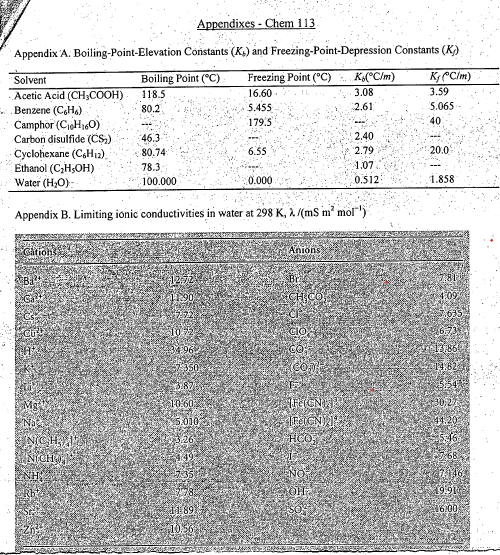
\includegraphics[width=0.75\textwidth, keepaspectratio]{images/151.png}
\end{center}



\item What is meant by limiting ionic conductivity? Explain why the limiting ionic conductivity of H$^+$ is so high compared to other cations. \mk{7}
\yr{CHEM 113 | 2015--16}



\item State Kohlrausch's law and Ostwald's dilution law. How can you use these two equations to determine the limiting values of the molar conductivity of solutions? \mk{9}
\yr{CHEM 113 | 2014--15}



\item For the reaction Ag(s) + $\frac{1}{2}$Cl$_2$(g) $\rightarrow$ AgCl(s), $E^\circ = 0.839$ V at 1000 K. If $a_{\text{Ag}} = a_{\text{AgCl}} = 1.00$ and $a_{\text{Cl}_2} = 0.77$, find the value of E. Is the reaction less favored under non-standard conditions? Justify from the values of $K$ and $\Delta G$. \mk{9}
\yr{CHEM 113 | 2013--14}



\item Define reversible cell. Give an example and explain how it is reversible. \mk{11}
\yr{CHEM 113 | 2011--12}



\item Establish a relation between the emf of a reversible cell and the heat of reaction in the cell. \mk{14}
\yr{CHEM 113 | 2011--12}



\item At 25$^\circ$C the value of the emf for the reversible cell: Pb, PbCl$_2$(s)$|$KCl(aq)$|$AgCl(s), Ag is 0.4902 volt and $(\partial E / \partial T)_p = -1.86 \times 10^{-4}$ volt$\cdot$deg$^{-1}$. Calculate the values of $\Delta G$ and $\Delta H$ showing the reaction involved in the cell. \mk{10}
\yr{CHEM 113 | 2011--12}



\item What are reversible and irreversible cells? Give one example of each. \mk{3}
\yr{CHEM 101 | 2009--10}



\item State the Kohlrausch law of independent migration of ions. Discuss its applications. \mk{9}
\yr{CHEM 101 | 2009--10}



\item Briefly discuss the chronological development of the mechanism of electrolytic conduction. \mk{8}
\yr{CHEM 101 | 2008--09}



\item Define transport number. Show that $t_+ + t_- = 1.0$. \mk{4}
\yr{CHEM 101 | 2008--09}



\item Explain the terms: conductance, specific conductance, equivalent conductance, and molecular conductance. Derive a relation between specific conductance and equivalent conductance. \mk{15}
\yr{CHEM 101 | 2007--08}



\item Give a brief description of the lead storage cell. \mk{10}
\yr{CHEM 101 | 2007--08}

%%══════════════════════════════════════════════════════════════════════
%% S9 — Polymers
%%══════════════════════════════════════════════════════════════════════
\item What is an electrochemical cell? How do you understand the terms ``half cell'', ``half-cell reaction'' and ``salt bridge''? \mk{10}
\yr{CHEM 101 | 2006--07}



\end{enumerate}
\newpage


\secdivider{Section S9}{Polymers}{cB}{cB}
\markboth{S9 --- Polymers}{}
\label{sec:S9}
\section{S9 --- Polymers}

\begin{enumerate}
\item Describe the mechanism of polymer conductivity. Discuss the effect of doping and other factors on the degree of conductivity. \mk{10}
\yr{CHEM 113 | 2023--24}





\item What are the different types of conducting polymers? Discuss the general mechanism of conduction in conjugated polymers. \mk{10}
\yr{CHEM 113 | 2022--23; 2020--21}



\item Show the chemical processes involved in doping polyacetylene and explain the increased conductivity of doped polyacetylene by discussing the mechanism of conduction in doped polymers. \mk{10}
\yr{CHEM 113 | 2022--23}



\item What distinguishes thermoplastics from thermosetting plastics? \mk{5}
\yr{CHEM 113 | 2021--22}



\item Apply your knowledge of intermolecular forces to explain the thermal transitions in amorphous and crystalline polymers. \mk{10}
\yr{CHEM 113 | 2021--22}



\item List the requirements of a conducting polymer for electrical conduction. Discuss a process for improving the conduction of polyacetylene, utilizing the concept of HOMO-LUMO. \mk{10}
\yr{CHEM 113 | 2021--22}



% extra
\item What are the different applications of conducting polymers? Discuss the general mechanism of conduction in conjugated polymers. \mk{10}
\yr{CHEM 113 | 2020--21}



\item ``The conductivity of doped polyacetylene is more than undoped molecule'' --- Justify by showing the addition of Lewis acid and Lewis base as dopant. \mk{10}
\yr{CHEM 113 | 2020--21}



\item Name the different types of polymerization processes with examples. \mk{5}
\yr{CHEM 113 | 2020--21}





%%══════════════════════════════════════════════════════════════════════
%% S10 — Electronic Materials
%%══════════════════════════════════════════════════════════════════════
\item What is thermoplastic starch? Discuss the applications and limitations of thermoplastic starch. \mk{10}
\yr{CHEM 113 | 2017--18}



\item Identify the factors that influence the biodegradability of polymers. Discuss the effect of crystallinity on biodegradability of polymers. \mk{10}
\yr{CHEM 113 | 2017--18}



\item Why are polymers often insulating? Draw energy level diagrams of metal, semiconductor and insulator. Indicate the band gaps and comment on their conducting behavior. \mk{10}
\yr{CHEM 113 | 2016--17}



\item How can polyacetylene act as a semiconductor? Draw energy level diagram of the hybridized p orbitals of a polymer consisting of conjugated double bonds and indicate their HOMO, LUMO, valence band and conduction band. \mk{10}
\yr{CHEM 113 | 2016--17}



\item Describe different types of doping mechanisms in conjugated polymers. What is the difference in the doping process of conjugated polymers and semiconductors? \mk{10}
\yr{CHEM 113 | 2016--17}



\item What are the factors that affect the conduction behavior of polymers? \mk{5}
\yr{CHEM 113 | 2016--17}



\item Why are natural polymers more biodegradable than synthetic polymers? What are the advantages, disadvantages and applications of thermoplastic starch? \mk{11}
\yr{CHEM 113 | 2016--17}



\item Write down the factors that accelerate the polymer degradation. \mk{9}
\yr{CHEM 113 | 2015--16}



\item Show schematically how a soliton pair on a trans-polyacetylene is formed by doping. \mk{6}
\yr{CHEM 113 | 2015--16}



\item How can a conjugated conducting polymer be doped by chemical methods? \mk{6}
\yr{CHEM 113 | 2015--16}



\item Write down the structures of the following polymers (any seven): (i) Poly(glycolic acid) (ii) Poly($\beta$-hydroxybutyrate) (iii) Poly-lysine (iv) Polyaniline emeraldine base (v) Polythiophene (vi) Polyazulene (vii) Poly($\epsilon$-caprolactone) (viii) Chitin \\(ix) Poly(dichlorophosphazene) (x) Starch. \mk{14}
\yr{CHEM 113 | 2015--16}


\end{enumerate}
\newpage

\secdivider{Section S10}{Electronic Materials}{cC}{cC}
\markboth{S10 --- Electronic Materials}{}
\label{sec:S10}
\section{S10 --- Electronic Materials}

\begin{enumerate}
\item Light-emitting diode (LED) is a modern innovation in digital display technology. Explain its mechanism that is different from LCD in producing a color band with a suitable diagram. Briefly state the characteristic features of LCD. \mk{10}
\yr{CHEM 113 | 2023--24}



\end{enumerate}
\newpage

%%══════════════════════════════════════════════════════════════════════
%% S11 — Biomolecules
%%══════════════════════════════════════════════════════════════════════

\secdivider{Section S11}{Biomolecules}{cD}{cD}
\markboth{S11 --- Biomolecules}{}
\label{sec:S11}
\section{S11 --- Biomolecules}

\begin{enumerate}
\item Protein is a bio-polymer --- explain by showing peptide bond formation. Explain the intermolecular forces responsible for stabilizing the secondary and tertiary structures of proteins. \mk{10}
\yr{CHEM 113 | 2023--24; 2021--22}



\item What can be inferred about the structure of DNA in terms of its double helix configuration and the complementary base pairing (A-T, G-C)? \mk{10}
\yr{CHEM 113 | 2021--22}




\item Explain the term ``Bile Salts''. Describe the types of interactions that are involved in maintaining the tertiary structures of proteins. \mk{15}
\yr{CHEM 113 | 2020--21 (Jan 21)}



\item How does hydrogen bonding and hydrophobic interaction influence the structure of biomolecules? \mk{10}
\yr{CHEM 113 | 2020--21}



\item Describe the forces that work efficiently to hold proteins in their most stable three-dimensional structures. Briefly explain the different ways in which protein structures could be unfolded. \mk{15}
\yr{CHEM 113 | 2019--20}



\item Draw the mechanisms of the acid hydrolysis of methyl-$\beta$-D-glucopyranoside. \mk{5}
\yr{CHEM 113 | 2017--18}



\item Draw the chemical structure of $\beta$-D-(+)-glucopyranose in chair conformation. Discuss the significance of $\beta$, D and (+). \mk{10}
\yr{CHEM 113 | 2017--18}



\item Define carbohydrates. Give one example of monosaccharides, disaccharides and polysaccharides. Draw their structural formulas. \mk{10}
\yr{CHEM 113 | 2016--17}



\item Draw the Fischer projection formula of D-glucose and L-glucose. \mk{5}
\yr{CHEM 113 | 2016--17}



\item Write down the mechanism of the formation of methyl glycoside from $\beta$-D-glucopyranose. Explain which anomeric product of methyl glycoside is more stable than the other. \mk{10}
\yr{CHEM 113 | 2016--17}



\item What is mutarotation? Why does glucose undergo mutarotation? \mk{5}
\yr{CHEM 113 | 2016--17}



\item Prove that glucose is a reducing sugar. \mk{5}
\yr{CHEM 113 | 2016--17}



\item Draw the primary, secondary, tertiary and quaternary structures of proteins. \mk{10}
\yr{CHEM 113 | 2016--17}



\item What sequence of bases on one strand of DNA is complementary to the sequence TATGCAT on another strand? \mk{3}
\yr{CHEM 113 | 2015--16}



\item ``Mutarotation occurs by a reversible ring-opening of each anomer to the open-chain aldehyde, followed by reclosure'' --- Explain with a suitable example. \mk{5}
\yr{CHEM 113 | 2015--16}



\item What do you mean by rRNA, tRNA and mRNA? What are the differences between DNA and RNA? \mk{9}
\yr{CHEM 113 | 2015--16}



\item Why are amino acids amphiprotic? Find out what species are present in a 1.00 M solution of alanine at pH = 9.00. The $pK_{a1}$ and $pK_{a2}$ values of alanine are 2.34 and 9.69, respectively. \mk{10}
\yr{CHEM 113 | 2015--16}




%%══════════════════════════════════════════════════════════════════════
%% S12 — Computational Chemistry
%%══════════════════════════════════════════════════════════════════════
\end{enumerate}
\newpage


\secdivider{Section S12}{Computational Chemistry}{cE}{cE}
\markboth{S12 --- Computational Chemistry}{}
\label{sec:S12}
\section{S12 --- Computational Chemistry}

\begin{enumerate}
\item What are the salient features of molecular mechanics in computational chemistry? Under what conditions or scenarios would you choose molecular mechanics as your preferred computational method? \mk{12}
\yr{CHEM 113 | 2023--24}



\item Draw a flow diagram illustrating the key stages of the modern drug discovery process. Explain how molecular docking is applied within this process. \mk{13}
\yr{CHEM 113 | 2023--24}




\item Write down the salient features of Density Functional Theory. Discuss the advantages and disadvantages of the Molecular Mechanics method. \mk{12}
\yr{CHEM 113 | 2022--23}



\item ``The accuracy of a calculation is dependent on both the model and the type of basis set applied to it'' --- Explain. \mk{10}
\yr{CHEM 113 | 2021--22; 2015--16}



\item What kinds of questions can computational chemistry answer? How are the different types of models used in computational chemistry? What advantages does computational chemistry have over ``wet chemistry''? \mk{20}
\yr{CHEM 113 | 2020--21 (Jan 21)}



\item What computable properties are studied by computational chemistry? Discuss the methods most commonly used in computational chemistry in terms of theories and cost (time) effectiveness. \mk{10}
\yr{CHEM 113 | 2020--21}



\item What precautions should one follow in computational chemistry? \mk{5}
\yr{CHEM 113 | 2020--21}



\item Discuss the importance of computational technology in drug delivery. \mk{15}
\yr{CHEM 113 | 2019--20}



\item How can computational chemistry be utilized to address real-world problems in chemistry? Briefly explain with specific examples. \mk{15}
\yr{CHEM 113 | 2019--20}



\item What do you mean by basis sets in computational chemistry? ``The accuracy of a calculation is dependent on both the model and the type of basis set applied to it'' --- Explain. \mk{6}
\yr{CHEM 113 | 2015--16}



\item Discuss the advantages and disadvantages of the Semi-empirical method of computation. \mk{5}
\yr{CHEM 113 | 2015--16}



\item Write down the salient features of the Ab-initio method. When would you choose this method for computation? \mk{7}
\yr{CHEM 113 | 2015--16}



%%══════════════════════════════════════════════════════════════════════
%% S13 — Miscellaneous
%%══════════════════════════════════════════════════════════════════════
\end{enumerate}
\newpage


\secdivider{Section S13}{Miscellaneous}{cF}{cF}
\markboth{S13 --- Miscellaneous}{}
\label{sec:S13}
\section{S13 --- Miscellaneous}

\begin{enumerate}
\item Explain why cis-1,2-dichloroethene has a higher boiling point compared to trans-1,2-dichloroethene. \mk{5}
\yr{CHEM 113 | 2023--24}




\item Draw a schematic diagram of the water desalination process and explain. \mk{10}
\yr{CHEM 113 | 2020--21 (Jan 21)}



\item Sea water contains dissolved salts at a total concentration of about 1.13 mol/L. Draw a desalination diagram for obtaining drinking water from sea water. \mk{6}
\yr{CHEM 113 | 2016--17}

% 

\item What is soap? Write down the mechanism of saponification of triacylglycerols. \mk{7}
\yr{CHEM 113 | 2016--17}



\item What is omega-3 fatty acid? Why is consumption of omega-3 fatty acid containing oils good for our health? \mk{7}
\yr{CHEM 113 | 2016--17}



\item What is soap? Show the cleaning mechanism of soaps. \mk{8}
\yr{CHEM 113 | 2015--16}



\item List four factors that can shift the position of an equilibrium. Which one can alter the value of the equilibrium constant? Why? \mk{8}
\yr{CHEM 113 | 2014--15}

\item The pH of a bicarbonate-carbonic acid buffer is 8.00. Calculate the ratio of the concentration of carbonic acid (H$_2$CO$_3$) to that of the bicarbonate ion (HCO$_3^-$). $K_{a1} = 4.2 \times 10^{-7}$. \mk{5}
\yr{CHEM 113 | 2014--15}

\item Define reaction quotient. How does it differ from equilibrium constant? What are the uses of reaction quotient? \mk{8}
\yr{CHEM 113 | 2014--15}

\item The equilibrium constant $K_c$ of the reaction N$_2$(g) + O$_2$(g) $\rightleftharpoons$ 2NO(g) equals $4.6 \times 10^{-31}$ at 25$^\circ$C. (i) What does the magnitude of $K_c$ tell you about the reaction? (ii) If you assume that the concentrations of N$_2$ and O$_2$ are 1.0 M, find the concentration of NO. \mk{9}
\yr{CHEM 113 | 2014--15}

\item At 128$^\circ$C the equilibrium constant ($K_c$) for the reaction Br$_2$(g) $\rightleftharpoons$ 2Br(g) is $1.1 \times 10^{-3}$. If the initial concentrations are [Br$_2$] $= 6.3 \times 10^{-2}$ M and [Br] $= 1.2 \times 10^{-2}$ M, calculate the concentrations of these species at equilibrium. \mk{10}
\yr{CHEM 113 | 2014--15}

\item What are the four variables or factors that can affect the rate of reaction? Which of the factor(s) affect the magnitude of the rate constant? Which factor(s) do not affect the magnitude of the rate constant? Why? \mk{8}
\yr{CHEM 113 | 2014--15}

\item The reaction of thioacetamide with water is shown by the equation below:
\[ \text{CH}_3\text{CSNH}_{2(\text{aq})} + \text{H}_2\text{O} \rightarrow \text{H}_2\text{S}_{(\text{aq})} + \text{CH}_3\text{CONH}_{2(\text{aq})} \]
The rate of reaction is given by the rate law: Rate $= k[\text{H}_3\text{O}^+][\text{CH}_3\text{CSNH}_2]$. Consider 1 L of solution that is 0.20 M in CH$_3$CSNH$_2$ and 0.15 M in HCl at 25$^\circ$C. (i) For each of the changes listed below, state whether the rate of reaction increases, decreases, or remains the same. Why? (A) A 4-g sample of NaOH is added to the solution. (B) 500 mL of water is added to the solution. (ii) For each of the changes listed below, state whether the magnitude of the rate constant $k$ will increase, decrease or remain the same. (A) A catalyst is added to the solution. (B) The reaction is carried out at 10$^\circ$C. \mk{8}
\yr{CHEM 113 | 2014--15}

\item The following values of the rate constant were obtained for the decomposition of nitrogen dioxide at various temperatures:
\begin{center}
\begin{tabular}{cc}
\toprule
Temperature ($^\circ$C) & $k$ (L/mol$\cdot$s) \\
\midrule
320 & 0.527 \\
330 & 0.776 \\
340 & 1.121 \\
350 & 1.607 \\
\bottomrule
\end{tabular}
\end{center}
Using the Arrhenius equation, determine the activation energy. \mk{10}
\yr{CHEM 113 | 2014--15}

\item The decomposition of hydrogen peroxide is a first-order reaction:
\[ \text{H}_2\text{O}_{2(\text{aq})} \rightarrow \text{H}_2\text{O}_{(\text{l})} + \tfrac{1}{2}\text{O}_{2(\text{g})} \]
The half life of the reaction is 17.0 minutes. (i) What is the rate constant of the reaction? (ii) If you had a bottle of H$_2$O$_2$, how long would it take for 86.0\% to decompose? (iii) If you started the reaction with $[\text{H}_2\text{O}_2] = 0.100$ M, what would be the H$_2$O$_2$ concentration after 15.0 minutes? \mk{9}
\yr{CHEM 113 | 2014--15}

\item Define (i) rate of reaction, (ii) rate of conversion, and (iii) rate constant. \mk{8--9}
\yr{CHEM 113 | 2013--14; 2010--11}

\item Define Hard and Soft Acids and Bases (HSAB). Discuss the classification of HSAB taking three examples from each class. \mk{10}
\yr{CHEM 113 | 2013--14}



\item Discuss the principle of application of HSAB in the following fields: (i) Medicinal Chemistry, (ii) Geochemical classification of the elements and their occurrence in nature as minerals, (iii) Predicting favorable equilibria, (iv) Toxicology. \mk{20}
\yr{CHEM 113 | 2013--14}



\item Explain why: (i) Picric acid is as strong as nitric acid though picric acid is an organic acid. (ii) Gold and copper are colored but silver is not, though they are elements of the same group IB. (iii) The coordination number of Co$^{3+}$ is six but that of Zn$^{2+}$ is four, though they are ions of `d' block elements. (iv) Potassium is more reactive than copper though they have 4s$^1$ electron in their outer shell orbital. (v) Transition metals generally form colored compounds. \mk{20}
\yr{CHEM 113 | 2013--14}



\item Define buffer solution. How does buffer solution work when small quantities of strong acid or base are added to it? \mk{16}
\yr{CHEM 113 | 2013--14}

\item Derive an expression for the rate of a first-order reaction which is opposed by another first-order reaction. How can you determine the equilibrium constant of such a reaction? \mk{17}
\yr{CHEM 113 | 2013--14}

\item In studying the decomposition of ozone $2\text{O}_3(\text{g}) \rightleftharpoons 3\text{O}_2(\text{g})$ in a two liter (2 L) reaction vessel, it is found that $\frac{d[\text{O}_3]}{dt} = -1.5 \times 10^{-2}$ mol$\cdot$L$^{-1}\cdot$s$^{-1}$. (i) What is the rate of reaction? (ii) What is the rate of conversion? (iii) What is the value of $\frac{d[\text{O}_2]}{dt}$? \mk{9}
\yr{CHEM 113 | 2013--14}

\item Explain why: (i) Bond in BeCl$_2$ is covalent but bond in CaCl$_2$ is ionic though Be and Ca are in the same group of the periodic table. (ii) Picric acid is as strong as nitric acid though picric acid is an organic acid. (iii) Gold and copper are colored but silver is not, though they are elements of the same group IB. (iv) The coordination number of Co$^{3+}$ is six but that of Zn$^{2+}$ is four, though they are ions of `d' block elements. (v) Potassium is more reactive than copper though they have 4s$^1$ electron in their outer shell orbital. (vi) Transition metals generally form colored compounds. \mk{24}
\yr{CHEM 113 | 2013--14}

\item Explain how a buffer solution resists the change in its pH value upon the addition of small quantities of strong acid or base. \mk{8--11}
\yr{CHEM 113 | 2012--13; 2011--12; 2010--11}

\item Define buffer solution and buffer capacity. \mk{6}
\yr{CHEM 113 | 2011--12; 2012--13}

\item What are Hard and Soft Acids and Bases (HSAB)? Explain the HSAB principle with examples. Mention the applications of hard and soft acids and bases concept. \mk{13}
\yr{CHEM 113 | 2012--13}

\item Discuss different classes of Lewis acids and bases. Cite two examples in each class. \mk{10}
\yr{CHEM 113 | 2012--13}

\item How will you determine the strength of acids and bases? Illustrate your answer with examples. \mk{12}
\yr{CHEM 113 | 2012--13}

\item Outline the significant features in the properties of the following pairs of molecules: (i) H$_2$O and H$_2$S, (ii) CO$_2$ and SiO$_2$, (iii) AgF and AgI. \mk{10}
\yr{CHEM 113 | 2012--13}

\item What are the differences between order and molecularity of a reaction? \mk{5}
\yr{CHEM 113 | 2012--13}

\item Show how you can determine the order of a reaction by the half-life method. \mk{6}
\yr{CHEM 113 | 2012--13}

\item Derive an expression for the rate constant of a first-order reaction. \mk{9}
\yr{CHEM 113 | 2012--13}

\item From the following data for the decomposition of N$_2$O$_5$ at 45$^\circ$C, show that the reaction is of the first order.
\begin{center}
\begin{tabular}{lrrrrrr}
\toprule
Time (min) & 0 & 10 & 15 & 20 & 25 & $\infty$ \\
Vol.\ of O$_2$ evolved (mL) & 0 & 6.30 & 8.95 & 11.40 & 13.50 & 34.75 \\
\bottomrule
\end{tabular}
\end{center}
\mk{12}
\yr{CHEM 113 | 2012--13}

\item Prove that buffer solution shows maximum buffer capacity when pH = pK. \mk{14}
\yr{CHEM 113 | 2011--12}

\item Define order of reaction. Show how you can determine the order of reaction by (i) half-life method and (ii) differential method. \mk{11}
\yr{CHEM 113 | 2011--12}

\item Derive an expression for the rate constant of a second order reaction. What are the characteristic features of a second order reaction? \mk{16}
\yr{CHEM 113 | 2011--12}

\item The decomposition of a gas follows second order kinetics. It takes 40 minutes for 40\% of the gas to be decomposed when the initial concentration is $4 \times 10^{-2}$ mol$\cdot$L$^{-1}$. Calculate the specific reaction rate. \mk{8}
\yr{CHEM 113 | 2011--12}

\item Establish the condition for maximum buffer capacity. \mk{12}
\yr{CHEM 113 | 2011--12}

\item Explain what is meant by the diagonal relationship. List two pairs of elements that show this relationship. \mk{8}
\yr{CHEM 113 | 2011--12}

\item What is buffer solution? How is it prepared? \mk{6}
\yr{CHEM 101 | 2010--11}

\item Prove that buffer solution shows maximum buffer capacity when pH = pK. \mk{14}
\yr{CHEM 101 | 2010--11}

\item Calculate the pH of a buffer solution consisting of CH$_3$COOH and 1.0 M CH$_3$COONa solutions. What will be the pH after the addition of 0.10 mol of HCl to one litre of this buffer solution? \mk{7}
\yr{CHEM 101 | 2010--11}

\item Discuss with example the principle of Hard and Soft Acids and Bases (HSAB) and also discuss one of its applications. \mk{8}
\yr{CHEM 101 | 2010--11}

\item Calculate the normality of 95\% (W/W) sulphuric acid solution of specific gravity (sp.\ gr.) 1.95 and also calculate the amount of water required per litre for this acid to convert its sp.\ gr.\ to 1.40. \mk{10}
\yr{CHEM 101 | 2010--11}

\item The reaction H$_2$ + Br$_2$ = 2HBr is carried out in a 0.250 L reaction vessel. The change in the amount of Br$_2$ in 0.01 s is $-0.001$ mol. (i) What is the rate of conversion? (ii) What is the rate of reaction? (iii) What are the values of $d[\text{H}_2]/dt$, $d[\text{Br}_2]/dt$ and $d[\text{HBr}]/dt$? \mk{9}
\yr{CHEM 101 | 2010--11}

\item Define rate law. Write the rate law for the following reaction: $a\text{A} + b\text{B} \rightarrow n\text{N} + m\text{M}$. \mk{10}
\yr{CHEM 101 | 2009--10}

\item What is a reversible reaction? Derive the rate expression for a first-order reaction opposed by another first-order reaction. \mk{15}
\yr{CHEM 101 | 2009--10}

\item The reaction SO$_2$Cl$_2 \rightarrow$ SO$_2$ + Cl$_2$ is a first-order reaction with the rate constant $2.2 \times 10^{-5}$ s$^{-1}$ at 302$^\circ$C. What percentage of SO$_2$Cl$_2$ will get decomposed in 90 minutes when the reaction is carried out at 302$^\circ$C? \mk{10}
\yr{CHEM 101 | 2009--10}

\item What is buffer solution? Classify buffer solution and show how they operate. \mk{9}
\yr{CHEM 101 | 2009--10}

\item Explain the terms `rate' and `rate constant' of reactions. \mk{8}
\yr{CHEM 101 | 2008--09}

\item Derive an expression for the rate constant of a second-order reaction involving one reactant only. What are the characteristic features of a second-order reaction? \mk{18}
\yr{CHEM 101 | 2008--09}

\item What are the modern concepts of acids and bases? Which one is the most acceptable concept in your opinion? Give reasons. \mk{12}
\yr{CHEM 101 | 2007--08}

\item Discuss five important bases for determining the relative acidity of different acids. Cite an example in each case. \mk{10}
\yr{CHEM 101 | 2007--08}

\item What are buffer solutions? How can they be classified? Show how a buffer solution functions. \mk{10}
\yr{CHEM 101 | 2007--08}

\item Derive the rate law for a first-order reaction being opposed by another first-order reaction. \mk{8}
\yr{CHEM 101 | 2007--08}

\item Derive and explain the Arrhenius equation. Show its application. \mk{16}
\yr{CHEM 101 | 2007--08}

\item For the decomposition of an acid, the value of the rate constant ($k$) at 0$^\circ$C is $2.46 \times 10^{-5}$ and at 30$^\circ$C is $1.63 \times 10^{-5}$. Calculate the energy of activation ($E_a$) of the process and comment on the result. \mk{11}
\yr{CHEM 101 | 2007--08}

\item What do you mean by the following terms used in chemical kinetics: (i) Order and Molecularity; (ii) Rate and Rate constant. \mk{10}
\yr{CHEM 101 | 2006--07}

\item Derive the integrated rate equation for the second order reaction $2\text{A} \rightarrow \text{P}$. Show how $t_{1/2}$ for such a reaction is dependent on the initial concentration. \mk{11}
\yr{CHEM 101 | 2006--07}

\item Describe two methods for the determination of the order of a reaction. \mk{6}
\yr{CHEM 101 | 2006--07}

\item The half-life period $t_{1/2}$ for a first-order reaction is 69.3 min at 27$^\circ$C and 34.7 min at 37$^\circ$C. Find out the energy of activation ($E_a$) for the reaction. \mk{3}
\yr{CHEM 101 | 2006--07}

\end{enumerate}

\end{document}